\documentclass[a4paper, 11pt]{article}

\usepackage[top = 2.5cm,
            bottom = 2.5cm,
            left = 2.2cm,
            right = 2.2cm]{geometry}
\usepackage{layout}
\usepackage{graphicx}
\usepackage{float}
\usepackage{array,booktabs}
\usepackage[style=numeric,sorting=debug,backend=biber]{biblatex}
\usepackage[T1]{fontenc}
\usepackage{todonotes}
\usepackage{paralist}
\usepackage{listings}
\usepackage{lmodern}
\usepackage{minted}
\usepackage[fleqn]{amsmath}
\usepackage{hyperref}
\usepackage[center]{caption}
\usepackage{multirow}
\usepackage{pbox}
\usepackage{arydshln}
\usepackage{amssymb}% http://ctan.org/pkg/amssymb
\usepackage{pifont}% http://ctan.org/pkg/pifont
\usepackage{titlesec}
\usepackage{rotating}

\newcommand{\sectionbreak}{\clearpage} % start each sec on new page

\setcounter{secnumdepth}{4}
\titleformat{\paragraph}
{\normalfont\normalsize\bfseries}{\theparagraph}{1em}{}
\titlespacing*{\paragraph}
{0pt}{3.25ex plus 1ex minus .2ex}{1.5ex plus .2ex}
\hypersetup{
  colorlinks,
  citecolor=black,
  filecolor=black,
  linkcolor=black,
  urlcolor=black
}
\usemintedstyle{autumn}
\lstset{language=SQL}
\addbibresource{report.bib}
\DeclareDatamodelEntrytypes{standard}
\DeclareDatamodelEntryfields[standard]{type,number}
\DeclareBibliographyDriver{standard}{%
  \usebibmacro{bibindex}%
  \usebibmacro{begentry}%
  \usebibmacro{author}%
  \setunit{\labelnamepunct}\newblock
  \usebibmacro{title}%
  \newunit\newblock
  \printfield{number}%
  \setunit{\addspace}\newblock
  \printfield[parens]{type}%
  \newunit\newblock
  \usebibmacro{location+date}%
  \newunit\newblock
  \iftoggle{bbx:url}
    {\usebibmacro{url+urldate}}
    {}%
  \newunit\newblock
  \usebibmacro{addendum+pubstate}%
  \setunit{\bibpagerefpunct}\newblock
  \usebibmacro{pageref}%
  \newunit\newblock
  \usebibmacro{related}%
  \usebibmacro{finentry}}
% Stop Latex from repositioning tables like an idiot
\restylefloat{table}

\begin{document}

\begin{titlepage}

\newcommand{\HRule}{\rule{\linewidth}{0.5mm}} % Defines a new command for the
% horizontal lines, change thickness here

\center

\vspace*{2cm}
\textsc{\LARGE Imperial College London}\\[1.5cm]
\textsc{\Large Department of Computing}\\[0.5cm]
\textsc{\large 3rd Year Group Project Report}\\[0.5cm]

\HRule \\[0.4cm]
{\huge \bfseries ATLAST}\\[0.6cm]
{\huge \bfseries Automatic Translation of Logic to}\\[0.2cm]
{\huge \bfseries ANSI SQL Tool}\\[0.4cm]% Title of your document
\HRule \\[1.5cm]

\begin{minipage}[t]{0.4\textwidth}
  \begin{flushleft} \large
    \emph{Authors:}\\
    Sean \textsc{Allan}\\
    Mitchell \textsc{Allison}\\
    Sam \textsc{Esgate}\\
    Thomas \textsc{Harling}\\
    Ted \textsc{Sales}\\
    Max \textsc{Tottenham}
  \end{flushleft}
\end{minipage}%
%
\begin{minipage}[t]{0.4\textwidth}
  \begin{flushright} \large
    \emph{Supervisor:} \\
    Dr. Fariba \textsc{Sadri}  % Supervisor's Name
  \end{flushright}
\end{minipage}%
\\[4cm]

{\large \today}\\[3cm] % Date, change the \today to a set date if you want to be precise

\vfill % Fill the rest of the page with whitespace

\end{titlepage}

\renewcommand{\contentsname}{\huge Contents \vspace{1cm}}
\tableofcontents
\clearpage

\setlength{\parskip}{0.3cm} \setlength{\parindent}{0cm}

\section{Executive Summary}
  \todo[inline]{A. Executive Summary 5\% of the whole project!

    Your 'elevator pitch'

    What is your Project? What does it do? Why would I want to buy it? etc.

    No implementation, software engineering details, or project management

Keep this short, see examples at

http://www.doc.ic.ac.uk/lab/thirdyear/group-project/last-year.html
}

  The overall project goal was to create a language translator which
  takes a restricted version of first-order predicate logic as input and
  produces the corresponding SQL as output. This allows any SQL relational
  database to be queried using only first-order predicate logic, without the
  user needing to know any SQL.

  The final implementation produced a lightweight and modular Python web
  application called ATLAST (Automatic Translation of Logic to ANSI SQL Tool)
  A minimalist web user interface allowed users to specify logic queries
  relating to any PostgreSQL database. The interface was augmented
  with poweruser features including predicate auto-fill and symbol shortcuts.
  Efficient code generation and SQL optimisation was handled by the server,
  which encapsulated logic queries as tasks to support multiple users through
  parallel translation by multiple backend servers.

  The primary use of the project was as a teaching tool for students taking
  logic and database courses. Students could practice writing logic sentences,
  and use the corresponding SQL produced to understand the meaning of the logic
  written and to view examples of correctly written SQL.

  Additionally, academics who are more used to writing logic than SQL, but who
  need to query a database as part of their research, can use the web app to
  greatly speed up their work. Where they would have previously been required to
  learn SQL, they can simply use our translation tool to save time. Finally,
  many SQL queries are far simpler and more understandable to write in logic.

\section{Introduction}

  \todo[inline]{Set the scene ... motivation'
  
  State the problem you are trying to solve ...objective(s)

  Summarise your main achievements}

  \subsection{Motivation}
    There are a number of groups and applications for which the project has
    clear use cases. Max felt there was a motivation for making this line longer
    or removing it.

    \subsubsection{Teaching}
      The predominant use-case for our project is as a teaching tool for use by
      students studying both logic and databases; topics which many universities
      deem mandatory for all computing students.
    
      To reinforce a student's understanding of logic, logic queries could be
      written and tested against a suitably populated database. The result of
      these queries can then be used to determine how well they have understood
      the course material, perhaps using an auto-checker against an expected
      result.

      As a further teaching method, the SQL generated by a student's input logic
      could be used as a reference for the student; either to highlight the
      meaning of their logic or to provide examples of correct and efficient
      SQL.     

    \subsubsection{Academic}
      Many academics are more accustomed to using logic within their work than
      writing SQL database queries. If an academic wanted to access data stored
      in a database as part of their research, large amounts of time could be
      saved if they could do this using familiar logic syntax.

      This would also remove the need to learn elemantary SQL, which they would
      use far less and be less proficient in. As academics may be unfamiliar
      with writing efficient SQL queries, the translator would likely produce
      more efficient SQL queries. This would be especially useful if querying
      large datasets.

    \subsubsection{Simplicity of logic over SQL}
\todo[inline]{Give examples of logic sentences that are far simpler to write and understand
compared to their SQL equivalent.}

    \subsubsection{Security (apparently!)}

    \subsubsection{Anything else you can come up with}

  \subsection{Objectives}
    The main objective was to provide a tool to translate first order predicate
    logic to a corresponding SQL representation. At the beginning of the
    project, it was decided that the key implementation goals would be:

    \begin{itemize}
      \item \textbf{Semantically correct translation from logic to SQL}

      \item \textbf{Simple and intuitive interface} that allows the user to
      efficiently learn and use the system

      \item \textbf{Support for user specified databases} without the need for
      further specialised or tedious configuration

      \item \textbf{Lightweight and easily deployable codebase} for reduced
      installation time and cost

      \item \textbf{Modular and expandable design} allowing fast updates and
      addition of new features
    \end{itemize}

  \subsection{Our solution}
    ATLAST is a web application that allows a user to select a database
    and query it using first order predicate logic. The logic is converted
    into corresponding SQL, which is then returned to the user, along with the
    result of running the query on the database.  
    
    The main achievements of the project were:

    \begin{itemize}
      \item \textbf{Creation of an SQL code generator} that is able to lexically
      analyse and parse user-input logic queries and generate ANSI SQL.

      \item \textbf{A minimalist front-end user interface} providing all
      translation funcitonaility from a single page, with clear links to
      support and database setup pages. Logic input shortcuts, including
      predicate auto-fill and logic symbol autocompletion, increase user
      productivity.

      \item \textbf{Server-side translation} provides queuing of translation
      tasks and assignment to multiple backend servers. Additionally, by the
      nature of connecting to a web app, users are always running the latest
      code and do not have to manually apply updates.

      \item \textbf{Provision of a database configuration utility} enabling
      users to specify the connection details of any PostgreSQL database, which
      the web application is then able to connect to and run queries on.

      \item \textbf{Small (less than 3MB) Python codebase} with minimal
      library dependencies. Installation time is on the order of ten minutes
      and requires no specialist programming knowledge.

      \item \textbf{Modularised architecture} to which specific code changes
      and updates can be quickly applied to individual sections including the
      GUI, lexer, parser or database support.
    \end{itemize}

\section{Background Research}
\label{sec:background}

\subsection{Datalog}
Before beginning the development of our project it was clear that there were strong links to Datalog. Datalog is a declarative logic programming language, resembling Prolog in syntax, that can be used to query deductive databases. Deductive databases are different from traditional relational databases in that new facts can be 'deduced' by applying rules to those facts already stored.

As an example, the following is possible in Datalog:
\begin{center}
  \begin{align*}
    &parent(jane, joe).     & grandparent(X, Y) :- parent(X, Z), parent(Z, Y). \\
    &parent(valerie, jane). & \\
  \end{align*}
  Left: Facts, Right: Rules 
  
  \begin{align*}
    &>> grandparent(A, B)?  & & >> parent(jane, C)? \\
    &>> A = valerie,        & & >> C = joe. \\
    &>> B = joe.            & & \\
  \end{align*}
  Deductions can be made when queried.
\end{center}

The fact $grandparent(Valerie, Joe)$ is not stored permanently but can be inferred at runtime, this is where the power of Datalog lies. Since there is no equivalent for this deduction in SQL and Datalog has been around since the 1970s we decided it would be an impossible challenge to out-develop it in a matter of weeks.

Rather than going head to head we realised that our project needed to approach the task from a different angle. Instead of requiring a database populated from the ground in a manner designed for logic queries we wanted to bring some of the benefits of logic to regular relational databases.
\begin{center}
  \begin{align*}
    & parent(jane, Child) & & \texttt{SELECT child} \\
    &                     & & \texttt{FROM people} \\
    &                     & & \texttt{WHERE parent = 'jane'} \\
  \end{align*}
  Which is nicer? Exactly.
\end{center}

\subsection{SQL}
  Structured Query Language (SQL)~\cite{wiki:SQL} is a special-purpose
  programming language designed for managing data held in relational database
  management system. SQL is made up of two different types of language:

  \begin{itemize}
      \item
        Data Definition Language. DDL is used to define the structure of a
        database (also known as its schema).
      \item
        Data Manipulation Language. DML is primarily used to insert, select,
        delete and update data within a database.
  \end{itemize}

  However, as defined by the SQL92 standard\cite{isoSQL}, read-only operations
  such as `SELECT' (without `INSERT INTO') should not exist as part of the DML;
  they do not manipulate the data, only query it. This distinction between
  read-only and read-write operations is not enforced, but here we will focus
  on read-only operations (so called 'SQL-data' operations) only.

  We initially chose to restrict to these operations so we could build a basic,
  but fully working system before progressing. Afterwards we considered how
  a statement that manipulates data, like an insert, could be defined in logic.
  \begin{gather}
    \top \rightarrow (film\_title(\$new, "Flight") \land film\_director(\$new, "James"))
  \end{gather}

  Above is one possibility, inserting a film called 'Flight', directed by 
  'James'. Having $\top$ imply the new information suggests that it must be 
  true, and if it doesn't currently hold it should be inserted. Problems here
  include automatically generating a primary key whilst keeping the syntax as true to
  logic as possible. Given time it would be possible develop this but for now
  it remains unimplemented.

\subsection{Tuple Relational Calculus}
  SQL was originally based on Relational Algebra and Tuple Relational
  Calculus. RA forms the structure and operations that can be performed
  across tuples of data and TRC provides a query language for such a model.

  \subsubsection{Formal Specification of Tuple Relational Calculus\cite{lecRA}}
    \label{sec:formalTRC}
    A query takes the form: \{T | p(T)\}. The answer of a query is said to be
    the set of all tuples T such that p(T) evaluates to true.

    A formula F is recursively defined as:
    \begin{itemize}
      \item $p(t_1, ..., t_n)$ where predicate $p$ is applied to terms $t_1, ..., t_n$ (atomic formula)
        \item $\lnot F$ where $F$ is a formula.
        \item $F' \land F''$ where $F', F''$ are formulae.
        \item $F' \lor F''$ where $F', F''$ are formulae.
        \item $\exists t(F)$ where $F$ is a formula and $t$ is a tuple of terms.
        \item $\forall t(F)$ where $F$ is a formula and $t$ is a tuple of terms.
      \end{itemize}

      $\exists t(F)$ is true if, for some tuple $t$ the formula $F$ is true. \\
      $\forall t(F)$ is true if, for all tuples $t$ the formula $F$ is true.

      A variable $v$ is bound in $F$ if it is of the form:

      $\exists t(F)$ or $\forall t(F)$ and $v \in t$.

      Otherwise $v$ is said to be free.
      
      Note that in query \{T | p(T)\} the variables in T must be the only
      free variables in p(T).

    \subsubsection{Querying Relational Algebra}
      Using all of this, it is possible to begin formulating some simple
      queries. For example, suppose it was desirable to query all films from a
      particular director in a database. It would be simple to write:

      \begin{center}
        \{F | F $\in$ Films $\land$ F.director = "Matt Damon"\}
      \end{center}

      This would however return all the elements of the tuple. The tuple may
      contain many irrelevant values to the user, and so it would be desirable
      to only return the title of said film. This could be achieved as detailed
      below:

      \begin{center}
        \{F | $\exists$F1 $\in$ Films(F1.director = "Matt Damon" $\land$ 
          F.title = F1.title)\}
      
        \emph{NOTE: F becomes a tuple with one element called title.}
      \end{center}

      We are now able to represent projection and selection. We can also
      represent joins. Let us suppose that we wish to find all titles of films
      whose director has also directed another film.

      \begin{center}
        \{F | $\exists$F1 $\in$ Films($\exists$F2 $\in$ 
        Films(F1.director = F2.director $\land$ F1 != F2)
        \\ $\land$ F.title = F1.title)\}
      \end{center}

\subsection{Mapping Tuple Relational Calculus to First-order Predicate Logic}
    \label{sec:tuplefo}
    With the knowledge of TRC, and how it underpins SQL, it is now necessary to
    formulate a mapping between TRC and first order predicate logic.

    \subsubsection{Atoms, Formulae, Predicates}
      Firstly atoms, formulae and predicates remain unchanged. We still wish to
      find a set of tuples that will result in a given formula evaluating to
      true.

    \subsubsection{Set Membership}
      Previously in TRC we could simply test the membership of a tuple $t$ in a
      relation $R$ with $t \in R$. First order predicate logic, at least in its basic,
      unsorted form, does not have the notion of variables belonging to
      different types or sets, they all belong to one global set. To solve
      this problem we propose a few solutions.

      One solution is with an `InRelation' predicate, where `InRelation(t, R)'
      would have the same semantic meaning as the previous set membership test.
      This seems to work, although throughout first order predicate logic, we
      do not have the notion of a tuple; an atom is structurally meaningless. A
      disadvantage of this would be that accessing members of the tuple would
      require another predicate, for example `InTuple(a, `attrName', t)' which
      would have the same semantic meaning as `t.a' in TRC.

      Another solution, which solves the previous issue, is to generate n-ary
      predicates that represent a tuple. For example, given a relation 'films',
      with columns `title', `length' and `date-released', a predicate
      `films(title, length, date-released)' could be generated, where title,
      length and date-released are all variables. This certainly solves the
      issue the set membership issue, but does add uneccessary bloat to each
      query; relations may have thousands of columns, very few of which are
      likely needed in a given query.

      The solution chosen addresses the issues raised so far.

      For a relation R(k, $a_{1}$, $a_{2}$, ..., $a_{n}$) with primary key k
      and n attributes we generate n + 1 predicates:
      \begin{align*}
        \text{1:  }     & R(k)           \\
        \text{2:  }     & R.a_1(k, a1)   \\
        \text{3:  }     & R.a_2(k, a2)   \\
                        & \vdots         \\
        \text{n + 1:  }  & R.a_n(k, an)
      \end{align*}
      Note: The predicate $R.k(k, k)$ is also valid, albeit redundant.

      Relating a tuple to its primary key gives a concise way to address it,
      adding the slight restriction that each relation must have a primary key.

    \subsubsection{Free and Bound Variables}
    \label{sec:freebound}

      Looking back to Tuple Relational Calculus in section~\ref{sec:formalTRC},
      we will use similar semantics for free and bound variables. Recall the
      syntax for the return value in TRC, the set of all tuples $T$, such that
      $p(T) \models \top$. Without extending predicate logic, we cannot use a
      similar format for specifying what is returned. However, all variables
      that are free in $p(T)$ must be in $T$ and so we assume that all unbound
      variables in the query are to be returned.

  \section{Translation of First-order Predicate Logic to SQL}

    Section~\ref{sec:tuplefo} provides a rough translation between
    first-order predicate logic and tuple relational calculus. From this
    grounding we can begin to define the mapping between logic and SQL.

    The examples in the section below will make use of the filmdb as used in
    the project. A description of the SQL schema can be found in the appendix,
    section ~\ref{sec:appfilmdb}.

    \subsection{Quantifiers}

    \subsubsection{Existentially Quantified Queries}

    Suppose we have the following first-order predicate logic query.
    \begin{gather}
      \exists x(films.title(x, title)) \label{select1}
    \end{gather}
    The query binds $x$ and leaves $title$ free, meaning that our
    answer will be the set of all subtitutions for $title$ such that
    $\exists x(films.title(x, title)) \models \top$. The `$\exists$' symbol
    serves two purposes. Firstly it binds $x$ as mentioned above, and secondly
    it enforces that the substituted $title$ exists in at least one tuple.
    The predicate $films.title$ gives the translator the scope of
    relations to query (in this case, just the $films$ relation).

    We can translate the query with use of the SQL SELECT statement. The SELECT
    statement is used to select data from a database\cite{w3SELECT}. Below is
    the translated query.
    \begin{minted}{sql}
    SELECT title
    FROM films;
    \end{minted}
    Strictly speaking since tuple relational calculus is based on set
    operators, like relational algebra, and SQL implcitly uses bag operators
    this actually evaluates to the following:
    \begin{minted}{sql}
    SELECT DISTINCT title
    FROM films;
    \end{minted}
    Note that it is perfectly valid to create a query with no bound variables,
    such as:
    \begin{gather}
      films.title(x, title) \label{select2}
    \end{gather}
    This will return the set of all tuples of the form \{$films.fid,
    films.title$\}, using the following SQL query.
    \begin{minted}{sql}
    SELECT fid, title,
    FROM films;
    \end{minted}
    Note that the DISTINCT keyword is no longer needed, as $films.fid$ is a
    primary key.

    Now we have demonstrated projecting a primary key, and a single attribute,
    all that is left is to project multiple attributes from a tuple. This
    requires the conjunction of multiple predicates, each over the same
    relation and using the same primary key (that is to say that each predicate
    relates to a single tuple). Suppose we wish to project
    every film title, and its corresponding length.
    \begin{gather}
      \exists x(films.title(x, y) \land films.length(x, z))
    \end{gather}
    As both $y$ and $z$ are from the same unique tuple identified by $x$
    (enforced by the conjunction within the query) our
    answer is equivalent to that returned by the following SQL query.
    \begin{minted}{sql}
    SELECT name, length
    FROM films;
    \end{minted}
    This can be extended to any number of predicates, although the relation and
    the key must be the same. If this is not the case, the query may represent
    a join, later described in section~\ref{sec:joins}.

    \subsubsection{Existentially Quantified Subqueries}
    \label{sec:existential}
    Often in a logical query, it will be common to existentially quantify a
    variable in an inner subquery. For example, the following subquery checks
    the existence of any films within our database with the same name, but that
    are not the same film, and returns the name of said film.
    \begin{gather}
      \exists x(films.title(x, title) \land \exists y(films.title(y,
      title) \land x != y))
    \end{gather}
    With a query of this format, we can simply translate the subquery, wrap it
    in an SQL EXISTS condition and conjunct this onto the WHERE clause of the
    outer query's query.

    \begin{minted}{sql}
      SELECT films1.title
      FROM films AS films1
      WHERE EXISTS (
        SELECT films2.title
        FROM films AS films2
        WHERE films1.fid <> films2.fid
      );
    \end{minted}

    There are two things to note with this approach, both relating to scope.
    The first is that the tables need to be aliased. SQL requires that aliases
    in subqueries must not have been used previously as the outer aliases are
    still in scope.
    
    The second is that in our logic $y$ is bound and we cannot make it free
    without changing the meaning of the query. If we cannot make it free
    then we cannot return it. Interestingly, in the SQL the outer scope cannot
    access fields in the inner scope, and so similarly cannot return it.
    Therefore we must create an exception to the free and bound variable rules
    that we specify in section~\ref{sec:freebound}.

    We could also repesent the previous query in a simpler form.
    \begin{gather}
      \exists x,y(films.title(x, title) \land films.title(y, title)
        \land x != y)
    \end{gather}
    This would translate to the following SQL query.

    \begin{minted}{sql}
    SELECT films1.title
    FROM films as films1 JOIN films as films2 ON films1.title = films2.title
    WHERE films1.fid <> films2.fid;
    \end{minted}

    Each of these forms are equivalent, and will return the same result.
    However, it is useful to be able to represent nested quantifiers, as it
    will not always be equivalent to combine them, for example in the case
    of implication, negation or duplicate variable names\cite{washEQUIV}.

    \subsubsection{Universally Quantified Variables}
    Using our knowledge from section~\ref{sec:existential}, we can now
    formulate a translation for universally quantified variables. In
    first-order predicate logic, the following equivalence holds:
    \begin{gather}
      \forall x(P(x)) \equiv \lnot \exists x(\lnot P(x))
    \end{gather}
    We can use this equivalence to simply encounter universally quantified
    variables as existentially quantified. Below is an example query in logic
    that aims to return all directors such that every film that they have
    directed is longer than one hour.
    \begin{multline}
      \exists x(films.director(x, director) \land \forall y(films.director(y,
      director) \\ \land films.length(y, length) \land length >
      \text{`1:00:00'}))
    \end{multline}
    We can think of this equivalently as following.
    \begin{multline}
      \label{eqn:except}
      \exists x(films.director(x, director) \land \lnot \exists y,length(\lnot(films.director(y,
      director) \\ \land films.length(y, length) \land length > \text{`1:00:00'})))
    \end{multline}

    Using De Morgan's laws, we can infer the following
    equivalence.
    \begin{multline}
      \label{eqn:demorganequiv}
      \lnot(films.director(y, director) \land films.length(y, length) 
      \land length > \text{`1:00:00'}) \\ \equiv (\lnot films.director(y,
      director) \lor \lnot films.length(y, length) \lor length \le \text{`1:00:00'})
    \end{multline}
    Equation~\ref{eqn:demorganequiv} however does not offer much progress, as
    we have not yet specified how to evaluate disjunction.

    Instead we must look to the query's semantic meaning. Referring to
    section~\ref{sec:except}, it can be seen that we need to make use of the
    SQL EXCEPT operator.

    We also must make use of the SQL EXISTS condition. The condition
    is used in a SQL query and is considered "to be met" if the subquery
    returns at least one row\cite{technetEXISTS}. The condition is useful in
    translating predicate logic to SQL, as it's meaning is consistent across
    both languages. 

    Our logical query now can be translated to the following SQL query.
    \begin{minted}{sql}
    SELECT film1.director
    FROM films AS films1
    WHERE NOT EXISTS (
      SELECT films2.director
      FROM films AS films2
      WHERE films2.director = films1.director
      EXCEPT
      SELECT films2.director
      FROM films AS films2
      WHERE films2.length > '1:00:00' AND films2.director = films1.director);
    \end{minted}

    \subsection{Equality}

      Suppose that we wish to check the existence of a film (The Bourne
      Identity) within our database. The constraint that the title must equal
      'The Bourne Identity' would be added to the WHERE clause, seen
      occasionally in previous sections. The WHERE clause is used to extract
      only those records that fulfill a specified criterion\cite{w3WHERE}.
      \begin{minted}{sql}
      SELECT title,
      FROM films
      WHERE title = 'The Bourne Identity';
      \end{minted}
      We expect to encounter at least one tuple if the film exists in our domain
      of discourse. This can be represented in one of two ways in first-order
      predicate logic.

      % This is two formulas, keep this as gather.
      \begin{gather}
        \exists x(films.title(x, y) \land y = \text{'The Bourne
        Identity'})\label{where1}\\
        films.title(x, \text{'The Bourne Identity'})\label{where2}
      \end{gather}
      Both of these queries are valid, however note that they do return different
      tuples. (\ref{where1}) returns the same answer as the SQL query above, although
      it is verbose. (\ref{where2}) returns the singleton tuple \{$films.fid$\},
      because under our definition, only free variables are returned. Most of
      the time this is acceptable, as it is often undesirable to return a
      constant term in the results, and also has the benefit of being more
      compact.

      So far we have used the notion of equality to bind variables to specific
      ground terms. We can also use equality to ensure that two variables have
      the same value. For example, consider the following logical query.
      \begin{gather}
        \exists a,b,y(actor.name(a, x) \land film.director(b, y) \land x = b)
      \end{gather}
      The query returns names of all of the actors who have also directed a
      film. This translates to the following SQL query. Ignore the cross join
      for now, this will be explained in section~\ref{sec:joins}.
      \begin{minted}{sql}
      SELECT name
      FROM actors CROSS JOIN film
      WHERE name = director;
      \end{minted}
      Note, that it is also possible to write the logic query in a more succint
      manner, as follows.
      \begin{gather}
        \exists a,b(actor.name(a, name) \land film.director(b, name))
      \end{gather}
      Here we have removed the equality constraint, instead unifying both
      predicates to the same variable. This is often a more desirable way to
      specify logical queries.

    \subsection{Inequality}

      Suppose that we wish to check the inverse of the previous section, that
      there exists other films except 'The Bourne Identity'. In SQL, this
      simply translates to the following.
      \begin{minted}{sql}
        SELECT title,
        FROM films
        WHERE title <> 'The Bourne Identity';
      \end{minted}
      The existence of one or more tuples satisfies our query; if no queries
      are returned, it must be the case that there are no other films except
      'The Bourne Identity'.

      As before, there are two ways we can represent the SQL query above in
      logic.

      % This is two formulas, keep it as gather.
      \begin{gather}
        \exists x(films.title(x, y) \land y !=  \text{'The Bourne
        Identity'})\label{where3}\\
        \lnot films.title(x, \text{'The Bourne Identity'})\label{where4}
      \end{gather}
      The first query matches the output of our equivalent SQL query, but again
      is more verbose. The second returns the set of singleton tuples
      \{$films.fid$\} such that the title associated with that particular
      primary key is not 'The Bourne Identity'. This is not equivalent to our
      SQL expression however, and may be undesirable to use in this
      circumstance (it is likely that we would like to return all other film
      titles).

      We can also express other inequalities, such as `<', `$\le$', `>', `$\ge$'.
      Here we query for all the fid of every films with length greater than or
      equal to two hours.
      \begin{minted}{sql}
      SELECT fid,
      FROM films,
      WHERE length >= '2:00:00';
      \end{minted}
      This can be expressed using the following predicate logic query.
      \begin{gather}
        \exists y(films.length(x, y) \land y \ge \text{`2:00:00'}) \label{where5}
      \end{gather}

      Queries can be constructed for the other inequalities in a
      similar manner.

    \subsection{Logical Connectives}

      It is often desirable to project a set of attributes from a statement
      made up of conditions and logical connectives. For example, suppose we
      wished to query the database for all film titles where the film is between 
      two and three hours in length. The relevant SQL query would take one of
      the following forms.
      \begin{minted}{sql}
      SELECT title
      FROM films
      WHERE films.length >= '2:00:00'
        AND films.length <= '3:00:00';

      SELECT title
      FROM films
      WHERE films.length BETWEEN '2:00:00' AND '3:00:00';
      \end{minted}
      This can simply be represented in first-order predicate logic with the
      following query.
      \begin{multline}
        \exists x, length(films.title(x, title) \land films.length(x,
        length)\\
        \land length \ge \text{`2:00:00'} \land length \le \text{`3:00:00'})
      \end{multline}
      Notice how the last two constraints in the logical query translate
      with very little effort. The same applies to constraints seperated with
      an $\lor$ which is equivalent to OR in SQL.

  \subsection{Conjunction of Predicates}
    \label{sec:joins}

    It is often desirable to use data spread across many relations in order to
    form useful queries. We can think of this simply in first-order predicate
    logic as the conjunction of predicates. When translating to SQL, retreiving
    data from multiple relation requires joins.

    An SQL JOIN clause is used to combine rows from two or more tables, based
    on a common field between them~\cite{w3JOINS}. Joins can enable incredibly
    powerful queries, especially where information
    is normalized (split across many relations) to minimise duplication.

    \subsubsection{SQL CROSS JOIN}

      A cross join is equivalent to the cartesian product of two sets. Suppose
      that we wished to write a query that returned every possible pair of
      film title and actor name in the database. In ANSI-89 SQL, we could use 
      the following query.
      \begin{minted}{sql}
      SELECT title, name
      FROM films, actors;
      \end{minted}
      Alternatively, in ANSI-92 SQL we can explicitly write:
      \begin{minted}{sql}
      SELECT title, name
      FROM films CROSS JOIN actors;
      \end{minted}
      We can think of this query as the conjunction of two disjoint relations;
      the relations do not share a key, or if they do we are not using them as
      part of the join.
      \begin{gather}
        \exists fid, aid(films.title(fid, title) \land actors.name(aid, name))
      \end{gather}
      The example used is unlikely to be a useful query on the database. Cross
      joins are rarely used in this format. Instead, they are often combined
      with a WHERE clause to extract useful information. For example, if we
      wished to query every actor that acted in the film 'The Bourne Identity',
      we could could use the following logic query.
      \begin{multline}
        \exists fid,cid(films.title(fid, \text{'The Bourne Identity'}) \\
        \land \land casting.fid(cid, fid) \land actors.cid(aid, cid) \land actors.name(aid, name))
      \end{multline}
      Which specifies that we only wish to return the set of all singleton
      tuples \{$actors.name$\} such that the actor starred in `The Bourne Identity'.
      With our knowledge of SQL CROSS JOIN, we can express this as the
      following SQL query.
      \begin{minted}{sql}
      SELECT name
      FROM films CROSS JOIN actors CROSS JOIN casting
      WHERE films.fid = actors.fid AND films.title = `The Bourne Identity' AND
      casting.fid = films.fid AND actors.cid = casting.cid;
      \end{minted}
      So far we have not discussed SQL aliases. Aliases are required if joining
      two instances of the same relation. To demonstrate this, suppose that we
      wish to generate the set of all pairs of actors that have appeared in the
      same film. This is achieved with the following SQL query.
      \begin{minted}{sql}
      SELECT a1.name,
             a2.name
      FROM films CROSS JOIN actors AS a1
        CROSS JOIN actors AS a2
        CROSS JOIN casting
      WHERE casting.cid = a1.cid AND casting.cid = a2.cid AND casting.fid =
      films.fid AND a1.name != a2.name
      \end{minted}
      Notice that we cannot simply refer to the relation $actors$ anymore, as
      there are two of them; without an alias, the identifier would be
      ambiguous. Below is a representation of the query in logic.
      \begin{multline}
        \label{largeCROSS}
        \exists fid, a1, a2(films(fid) \land casting.fid(cid, fid) \land
        actors.cid(a1, cid) \land actors.cid(a2, cid) \\
        \land actors.name(a1, name1) \land actors.name(a2, name2) \land name1 != name2)
      \end{multline}

    \subsubsection{SQL INNER JOIN}

      Introduced in ANSI-92 SQL, INNER JOIN allows for a more readable version of
      the above CROSS JOIN, WHERE combination. The logical query~\ref{largeCROSS}
      can be written using the SQL INNER JOIN syntax as:

      \begin{minted}{sql}
      SELECT a1.name,
             a2.name
      FROM films CROSS JOIN actors AS a1
        CROSS JOIN actors AS a2
      ON films.fid = a1.fid AND films.fid = a2.fid 
        AND a1.name != a2.name
      \end{minted}

      INNER JOIN is the same as JOIN as of ANSI-92 SQL. The existence of
      the ON clause is not necessary (making it a cross join).

    \subsubsection{Translating to the Correct Join}

      Fundamentally, joining two relations often occurs as the result of a
      conjunction of predicates when translating from first-order predicate
      logic. However, there are a few different circumstances which affect the
      type of join that must be used. Table~\ref{table:jointranslation} explains
      the different types of join that can result from a query.

      \newcommand*{\tabbox}[2][t]{%
            \centering\vspace{0pt}\parbox[#1][3.7\baselineskip]{6.5cm}{\strut#2\strut}}

      \begin{table}
        \begin{tabular}{ | 
          p{\dimexpr 0.5\linewidth-2\tabcolsep} |
          p{\dimexpr 0.5\linewidth-2\tabcolsep} |
        }
        
        \hline
        Dilemma & Explanation \\
        \hline

        \tabbox{\centering $rel.attr1(k, a) \land rel.attr2(k, b)$ \\ becomes \\  No Join} 
        & 
        Both keys and relations are equal. This conjunction involves projecting
        two elements from the same tuple, and so no join is necessary.
        \\\hline
        
        \tabbox{\centering $rel1.attr1(k1, a) \land rel2.attr2(k2, b)$ \\ becomes \\ CROSS JOIN} 
        & 
        The keys are different and the relations may or may not be equal. Since
        we assume that a != b, there are no common elements, and a cross join
        must occur.
        \\\hline
        
        \tabbox{\centering $rel1.attr1(k1, a) \land rel2.attr2(k2, a)$ \\ becomes \\ JOIN ON \\ rel1.attr1 =
        rel2.attr2} 
        & 
        The keys are different, but the attributes rel1.attr1 and rel2.attr2
        are equal, thus we must join on these elements. Note that aliases are
        used to avoid ambiguity between the two sets of attributes if they
        overlap.
        \\\hline
        
        \tabbox{\centering $rel1.attr1(k, a) \land rel2.attr2(k, b)$ \\ becomes \\ JOIN ON \\ rel1.key =
        rel2.key}
        & 
        The keys are the same and we assume the attributes rel1.attr1 and rel2.attr2
        are different. We must join on the keys. Note that aliases are
        used to avoid ambiguity between the two sets of attributes if they
        overlap.
        \\\hline
        
      \end{tabular}
        \caption{How logic relates to joins. Rules can combine to create more
        complex joins.}
        \label{table:jointranslation}
    \end{table}

  \subsection{Negation}

    \subsubsection{Difference}
    \label{sec:except}

    It may be the case that we need to negate a set of predicates. By example,
    we will refer to the subquery within
    equation~\ref{eqn:except}:
    \begin{align*}
      \exists y,& length( \\
      &\lnot(films.director(y, director) \land films.length(y, length) \land length > '1:00:00') \\
      ) \hspace{2mm} &
    \end{align*}
    Semantically, we wish to prove that a y exists, such that y is the films
    fid, and the length of that film is above one hour. We could formulate the
    translation as below:
    \begin{minted}{sql}
    SELECT films.director
    FROM films
    WHERE length <= '1:00:00';
    \end{minted}
    So the answer is simply achieved by negating the condition. However, if
    there are other constraints in the query that create a join, we do not wish
    to negate these; we only wish to negate the conditions that restrict the
    data after a join. The simplest method here to solve this problem is to use
    the EXCEPT operator.

    The SQL EXCEPT operator takes the distinct rows of one query and returns
    the rows that do not appear in a second result set\cite{wiki:EXCEPT}. It
    has the same semantic meaning as the set difference operator. The
    above SQL query is equivalent to the following.

    \begin{minted}{sql}
    SELECT films.director
    FROM films
    EXCEPT
    SELECT films.director
    FROM films
    WHERE length > '1:00:00';
    \end{minted}

  \subsubsection{NULL Values}
    The SQL language implements three-valued logic. A condition can either
    translate to TRUE, FALSE or UNKNOWN.

    Often in relations, it will be common to come across a NULL value. A NULL
    value can represent any of the following\cite{pmbNULL}:

    \begin{itemize}
      \item NULL represents a something that is not present in the UoD
      \item NULL represents something that might be present in the UoD, but
        we do not know its value at present
      \item NULL represents something that is present in the UoD, but we do
        not know its value at present
    \end{itemize}

    In our implementation, we will take NULL to be the second representation.

    This is particularly useful because it allows us to postulate questions like
    the following "List the names of all films who's director is not known" as:
    \begin{gather}
      \exists x(films.name(x,name) \land \lnot films.director(x, director) )
    \end{gather} 
    It is common for SQL queries to check if a value is NULL, as the user may
    wish to exclude these values, or perform a special case if they are
    encountered.

\section{Design and Implementation}
  \subsection{Application Type}
    We wanted a system that was easy to set up and worked on any operating
    system. The first point of discussion was whether a desktop client or a web
    application would be better suited.

    \begin{center}
      \renewcommand{\arraystretch}{1.5}%
      \begin{tabular}{ r | l | l }
        \multicolumn{1}{c |}{\textbf{Feature}} &
          \multicolumn{1}{c |}{\textbf{Desktop Client}} &
          \multicolumn{1}{c}{\textbf{Web Based}} \\
        \hline
        \emph{Processing}     & \ding{51} Local (Low Latency) & \ding{55} Remote (High Latency) \\
        \emph{Interface}      & \ding{51} Native              & \ding{51} Universal \\
        \emph{Multi-Platform} & \ding{55} Difficult           & \ding{51} Easy \\
        \emph{Installation}   & \ding{55} Required            & \ding{51} None \\
        \emph{Updates}        & \ding{55} Manual              & \ding{51} Automatic \\
      \end{tabular}
    \end{center}

    It is worth noting that using C++ and Qt would have mitigated some of the
    problems with desktop clients. Qt is a development framework that allows
    you to develop for Windows, Mac OS X and Linux simultaneously. This was
    appealing because we didn't want to limit ourselves to one platform but at
    the same time didn't have the time to develop three separate versions. Even
    taking all of this into account we felt that a web based system made more
    sense.

    Whilst C++ and Qt was supposedly cross-platform, it came with a few caveats,
    namely that you had to write proper cross-platform C++ code, adding an extra
    complication to our development. Additionally, Qt is not strictly cross
    platform; the huge variety mobile device platforms with app stores makes
    development even more complex. In contrast, a web interface is almost
    guaranteed to work on any device that has a browser, which we believed was a
    more relevant scope of devices and users.

  \subsection{Language Choice}
    Given our interface choice, we clearly needed to develop a front end using
    the traditional combination of HTML, CSS and JavaScript, (or variants of
    these) but what to choose for the backend? We didn't want anything
    complicated, just a simple web server to accept requests and
    a way of sending these requests on for processing. Using something like C
    for this was overkill - we wanted to be able to quickly prototype and
    experiment. As such, three languages came to mind.

    \begin{center}
      \renewcommand{\arraystretch}{1.5}%
      \begin{tabular}{r | l | l | l}
        \multicolumn{1}{c |}{\textbf{Feature}} & \multicolumn{1}{c |}{\textbf{Python}} & \multicolumn{1}{c |}{\textbf{Java}} & \multicolumn{1}{c}{\textbf{Ruby}}\\
          \hline
          \emph{Complexity of Language} & \ding{51} Simple      & \ding{55} Average   & \ding{51} Simple \\
          \emph{Previous Experience}    & \ding{55} None        & \ding{51} Lots      & \textbf{-} Some \\
          \emph{Plugin Support}         & \ding{51} Good        & \ding{51} Good      & \ding{51} Good \\
          \emph{Compilation (Speed)}    & \ding{51} Interpreted & \ding{55} Compiled  & \ding{51} Interpreted \\
      \end{tabular}
    \end{center}

    Java was the first to be eliminated, even though all group members had
    experience using it, mainly because development in general takes longer when
    compared with Ruby or Python. Though it's much easier to write than say C,
    it lacks features like dynamic typing which make rapid prototyping easier.

    There was little to choose between Python and Ruby, both are garbage
    collected, dynamically typed and concise languages. We had used Ruby in our
    previous work and it was decided, simply out of curiosity, that we would try
    Python.

  \subsection{Architecture}
    \begin{figure}[h!]
      \centering
      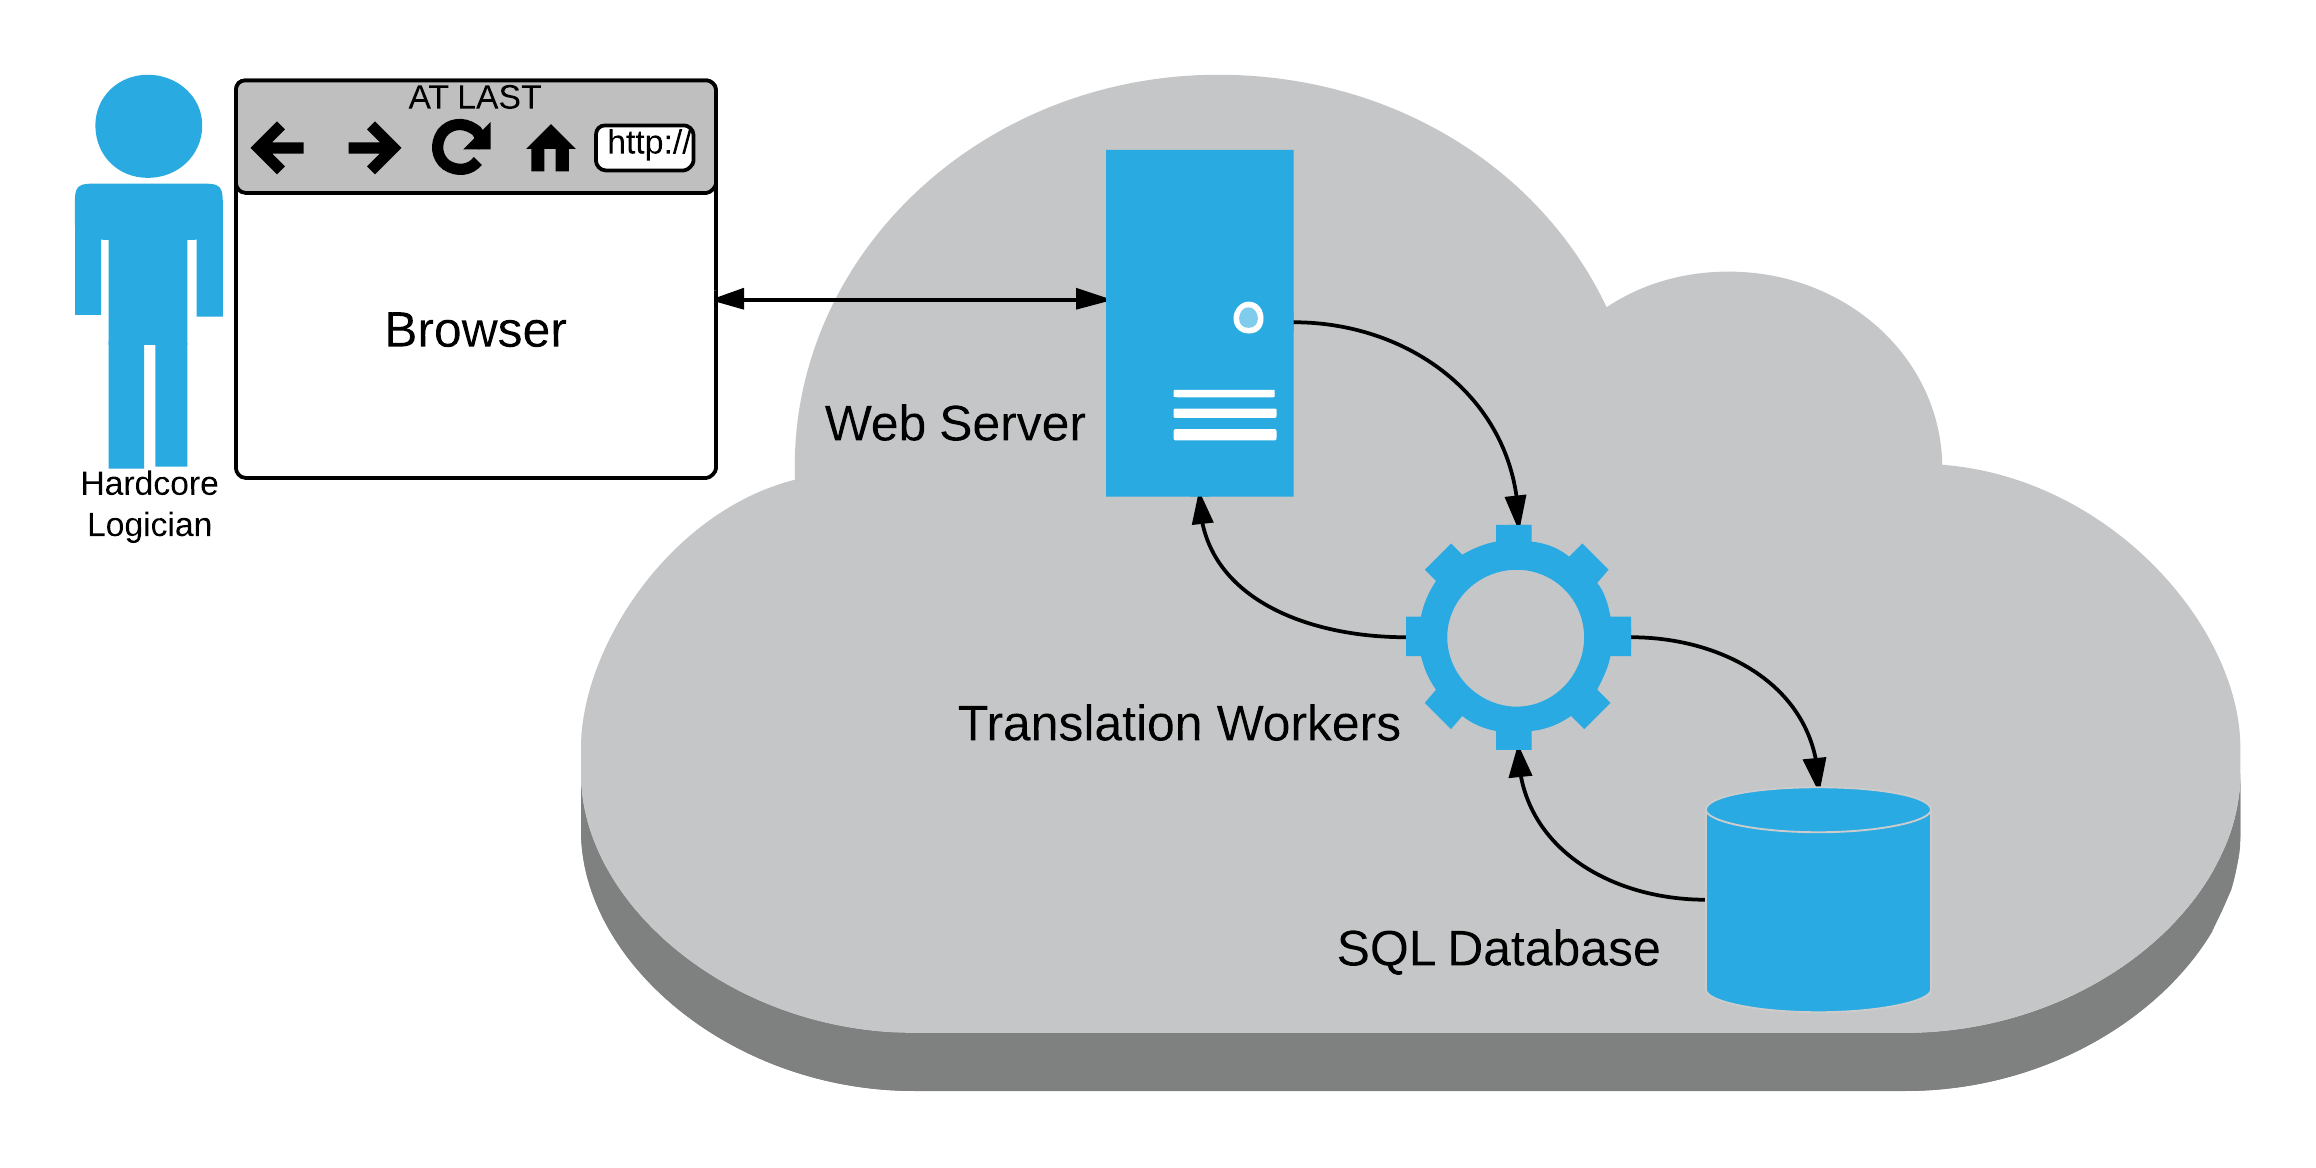
\includegraphics[width=\textwidth]{images/architecture.png}
      \caption{High-level system architecture diagram}
    \end{figure}
    With all this in mind, we designed a high-level architecture of ATLAST. One
    key consideration was the separation of various sections and services, in
    order to allow future expansion and flexibility. For example, the system
    should be able to change what database server it was connecting to, or to
    send off translation requests to various services for load-balancing and
    scalability.

    From this concept we were able to split the system up into three areas - the
    front end, the middleware, and the back end. The front end was the user's
    interface into the system, i.e. the browser experience. The back end
    consisted of the core operational components that did the actual translation
    of logic to SQL, and to interface with the database. The middleware then
    links these two parts together with a web service to host the front end and
    a method of managing the back end's translation processes, allowing both to
    communicate with each other.

  \subsection{Front End}
    \subsubsection{Graphical user interface}
      \begin{figure}[h!]
        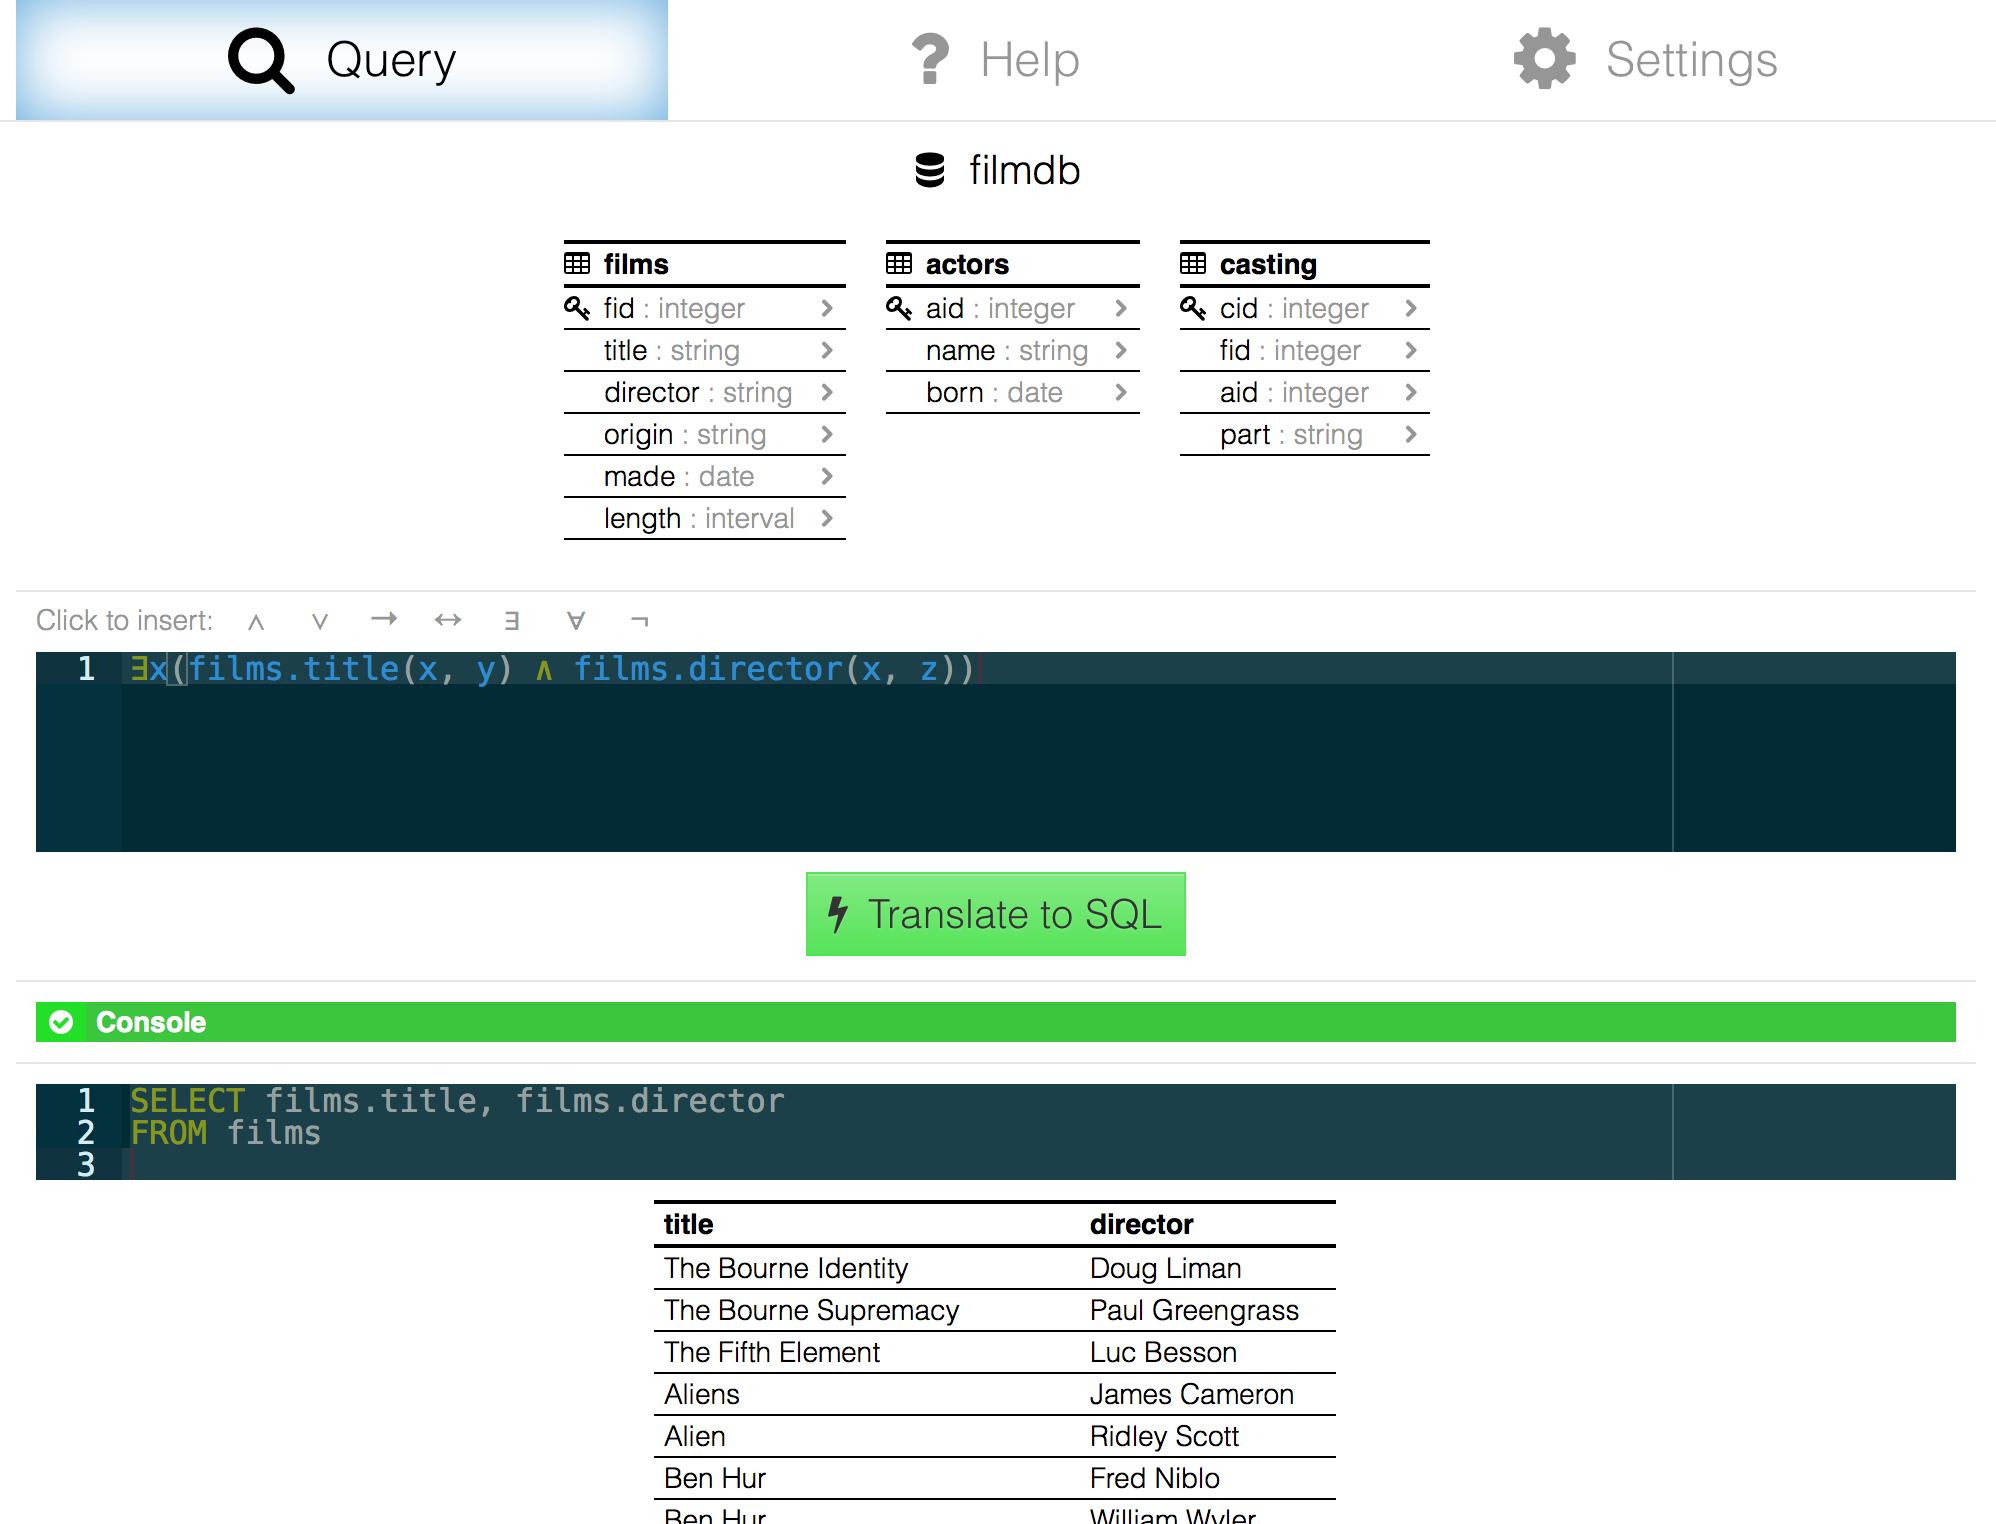
\includegraphics[width=\textwidth]{images/site_query.png}
        \caption{Main `Query' page}
      \end{figure}
      The interface that the user would see and interact with had to be simple
      and intuitive to use. In particular, this meant that logic queries had to
      be easy to input and the resulting SQL with the result of running it on
      the database had to be clear and understandable.

      The site was designed with the fewest number of pages possible, in order
      to maintain its simplicity and ease of use. When a user browses to the
      site, the homepage is the logic translation page. This allows the user to
      begin working straight away, with no setup costs or many pages to first
      browse through.

      As such we designed an easy way of inputting common logic symbols and
      operators, with the view that doing so with a keyboard would be very
      difficult in many cases, particularly as half of them are not present on
      standard keyboards. This reduced the entry barrier for potential users -
      what could be easier than clicking on a symbol to insert it?

      Information about the database schema was prominently displayed at the top
      of the query page. The data included the database name, table names, table
      attributes, attribute types and marking of key attributes. This makes the
      structure of the database very obvious, and an extra feature of this was
      the addition of buttons for each attribute. These buttons would insert
      into the logic query the predicate corresponding to the chosen attribute,
      reducing syntax errors due to spelling mistakes, requiring the user to
      type less to achieve their desired query.

      In addition to the translation page, there is also a help page and a
      settings page. The help page provides an easy to understand guide on how
      to write and form logic queries, whilst the settings page allows the user
      to specify their own database to connect to and run queries on. The links
      to these two pages are placed at the top of the page in the form of tabs,
      so that they are easily accessible.

      We also implemented syntax highlighting for predicate logic in our input
      box, which aids readability and helps the user know when their syntax is
      incorrect.

      Another power feature we created was a method of easily inserting logic
      symbols using just the keyboard. This was implemented by using typed
      character sequences that corresponded to various logic symbols, for
      example the sequence `<->' would be replaced with the unicode character
      $\leftrightarrow$.

    \subsubsection{HTTP REST and JSON}
      The user interface's communication with the web server was based on the
      REST principle~\cite{rest}. This involved sending and receiving JSON with
      the web server to perform various tasks.

      The database schema could be requested performing a GET request to
      `/schema'. A POST request to `/' was used to send the logic string to the
      web server for translation using the AJAX principle, where the browser
      sends an asynchronous HTTP request and does not refresh the page.

      The JSON data format was also used to transfer the logic input by the user
      to the server, and the translated SQL to the user from the server. The
      format was chosen as it is parsed automatically by the browser into
      native JavaScript objects. This made the interface between the server and
      the client very smooth and simple.

    \subsubsection{Plugins and Libraries}
      The site made heavy use of jQuery~\cite{jquery}, a very common JavaScript
      library which makes common tasks much more straightforward, to speed up
      development and yield a more engaging user experience. Other libraries are
      available for this purpose such as MooTools~\cite{mootools}, but our
      experience with jQuery in the past made the choice for us.

      The Ace~\cite{aceEditor} code editor was used as the input box for the
      user's logic query. The editor was both extremely powerful and very
      customisable, whilst being fairly straightforward to integrate into the
      existing codebase.

      The editor provided a familiar interface when compared with desktop
      applications such as Vim or Sublime Text, and the colour scheme could be
      changed to commonly used themes available from these existing editors.

      The editor had a number of advantages over using a simple HTML textarea.
      This included line numbers, but also syntax highlighting. This was
      achieved by creating a `mode' for the editor to use, with a set of
      highlighting rules that govered how the input was split into tokens. These
      tokens would represent various elements in the predicate logic language,
      such as variables, logic symbols or predicates.

      The highlighting rules were based around a state machine which acted much
      like an LL(1) parser. This meant our existing LALR(1) parser grammar could
      be adapted to work with the syntax highlighting rules. This took a bit of
      time but yielded excellent results, as can be seen above.

  \subsection{Middleware}
    \subsubsection{Web Server}
      The web.py framework~\cite{webpy} was chosen to host the user facing site.
      Doing so allowed us to quickly set up a functioning site and concentrate
      on developing useful features, instead of spending a large amount of time
      setting up a more complicated web server.

      We seriously considered Django as an alternative web framework, but we
      were put off by its complex configuration and its focus on
      enterprise-level features. For example, it was not trivial to host static
      pages or media like images with Django, for no obvious reason. It was this
      that persuaded us to go with a far lighter framework, such as web.py.

    \subsubsection{Celery and RabbitMQ}
      By default web.py is multi-threaded, meaning that each users request is
      handled in a separate thread. This allows multiple users to send HTTP
      requests to the server at once.

      Because of this, it would indeed be possible to run the translation code
      in the same thread that services a user's request. However in an effort
      to make our project scalable we decided to use a 3 tiered architecture.

      To achieve this, the Celery~\cite{celery} asynchronous task queue and
      RabbitMQ~\cite{rabbitmq} message broker were used. Each logic sentence to
      translate could be easily packaged into its own task and added to a queue
      to be translated.

      A user makes a request to the web server, the web server dispatches a job
      to RabbitMQ, a Celery worker listens to the RabbitMQ task queue and when a
      new job arrives, it pulls it off the task queue, processes it and posts
      the result back to RabbitMQ. Here RabbitMQ is acting as a message broker
      for the server to communicate to the Celery worker. Currently our
      implementation assumes that all three services are running on the same
      machine, however it is very easy to edit the configuration so that the
      platform can scale to an arbitrary number of separate workers on different
      physical devices.

      Below is an example of how these services are used in our project:
      \begin{minted}{python}
        # In file code.py
          import task as worker
          result = worker.addToProcessingQueue.delay(logic, web.schema, web.config)
          response = result.get()

        # In file worker.py
        @celery.task
        def addToProcessingQueue(logic, schema, configData):
          # Logic translation here
      \end{minted}

    \subsection{Logic to SQL translation}
      In this section, we will focus on the implementation of the translation
      between first-order predicate logic and SQL.

      The problem can be broadly thought of as the translation of a source
      langauge into a target language, a task that is commonly performed by
      compilers. Another alternative would have been to create an interpreter.
      Interpreters are very similar to compilers, in that they manage the
      translation from one language to another, but instead of translating the
      whole program into machine code, they create an intermediate
      representation, and then translate and execute the representation at
      runtime.

      We chose to create a compiler for two reasons. The first was that a
      logical query is not useful if part of it is malformed. In an interpreted
      language, an expression that is malformed but not executed is allowed to
      exist. The second was mainly due to the previous experience of the group
      members, all of whom have studied a Compilers course.

      We used the PLY library, which is an implementation of GNU's LEX and YACC
      written in Python, in order to generate a parser and lexer for our
      project.
    \subsubsection{Lexical Analysis}

      First we specify the tokens that make up the lexical stage of parsing
      using regular expressions. This can be seen in
      \texttt{lexer.py}. PLY automatically identifies something as a token if it
      has the following format: \texttt{t\_TOKENNAME}

      It can either be a constant, or for more complex tokens such as
      identifiers it can be a function.
      The lexer is generated by calling ply.lex.lex(). The lexer splits the
      source language (in this case, the logical query) into these tokens that
      can then be analysed in the parsing stage.
  
      \begin{center}
        \begin{minted}{python}
          t_LBRACKET = '\('
          t_RBRACKET = '\)'
          t_COMMA = ','
          t_NOT = u'\u00AC'

          digit = r'([0-9])'
          nondigit = r'([_A-Za-z])'
        \end{minted}
        Example Tokens, in their natural environment. 
      \end{center}

      \todo{Maybe, natural environment isn't the right phrase.}

      \subsubsection{Building an Abstract Syntax Tree}

      The logic queries that we parse form an LALR(1) (Look-Ahead, Left to
      right, Rightmost deriviation) grammar\cite{sittingacrossthere}. The
      grammar is described in \texttt{parser.py} in a notation similar to BNF.
      PLY's implementation of YACC requires you to define your rules as a
      python docstring. PLY then parses the docstring to generate a full
      representation of the grammar, calling the defined functions as
      necessary. A parameter to the function is $p$, an array where $p[i]$
      holds the value of the i\textsuperscript{th} (1-indexed) token or state matched in the
      grammar. The function should leave the resolved state object in $p[0]$.
      As an example, the following function specifies the rule for a bracketed
      $formula$, which resolves simply to the $formula$ state. 
      \begin{minted}{python}
        def p_formula_bracketed(p):
          'formula : LBRACKET formula RBRACKET'
          p[0] = p[2]
      \end{minted}

      As the grammar is reduced, an abstract syntax tree is built from the
      bottom up. The AST is made up of \texttt{Node} subclasses found within
      the \texttt{ast/}
      directory. Each subclass will contain its own internal representation of
      the language construct, but most follow the general convention of having
      a number of children nodes.

      For example, take the simple logical query below:
      \begin{multline}
        \exists x(films.title(x, y))
      \end{multline}

      This will build the following abstract syntax tree.

      \todo{Create simple AST graphic}

      Below you can find a more complex reduction rule, a more complicated
      logical query and its resulting AST:

      \begin{minted}{python}
        ### A /\ B ###
        def p_formula_and(p):
          'formula : formula AND formula'
          lineNo = p.lexer.lineno
          pos = getPosition(p.lexer)
          p[0] = ast.AndNode(lineNo, pos, p[1], p[3])
      \end{minted}

      \begin{gather}
        \exists x(films.title(x, y) \land films.director(x, z))
      \end{gather}

      \todo{Create more complex AST graphic}

      At the end of the parsing stage, the root
      node will be accessible to then perform symbol table, and later code,
      generation.

    \subsubsection{Generating a Symbol Table}

      Now that a well formed AST has been constructed, the tree is then
      traversed, populating a symbol table. Here we take the meaning of a
      symbol table to be similar to that of a compiled object file, a structure
      that holds information needed to locate and relocate a program's symbolic
      definitions and references.\cite{symtab}

      Below are justifications for the use of a symbol table.

      \paragraph{Scoping}
        In a logic query, is is possible to reuse variable names in an inner
        scope that exist in an outer scope. For example, take the following
        query in logic.
        \begin{multline}
        \exists x(films.title(x, y) \land \forall x(films.title(x, y) \land
        films.length(x, z) \land z > '1:00:00)) \label{eqn:scoping}
        \end{multline}
        This query returns the set of all singleton tuples $\{films.title\}$ such
        that for all films with the same title, they all are longer than one
        hour. Note that we quantify $x$ twice, once with an existential
        quantifier and once with a universal quantifier. For this reason, the
        inner subquery's definition of x is different to the outer subquery's.
        For this reason, we must be able to distinguish between different
        scopes. This can be achieved by using a hierarchical symbol table.

      \paragraph{Unification}
        Similarly, if two variables are in the same scope, it is important that
        they are unified; both variables should refer to the same underlying
        value. Referring back to equation~\ref{eqn:scoping}, even
        though $y$ exists within both scopes, because it is not redefined
        within the inner scope, each instance of the variable refers to the 
        same value.

      \paragraph{Free and Bound Variables}
        We typically rely on a variable being defined by a quantifier, but
        there are many occasions where this is not the case. Referring back to
        equation~\ref{eqn:scoping} again, we see that $y$ is returned as it a
        free variable, a convention that was agreed on back in
        section~\ref{sec:freebound}. As $y$ has not been defined before, it is
        necessary to add the declaration of $y$ into the symbol table, in a top
        level 'global scope'. This way, any redeclarations of $y$ are caught
        lower in the table, but any instance of $y$ that exists outside of a
        scope in which it has been redeclared will have a reference to this
        global instance.

      The symbol table structure is defined in the file
      \texttt{codegen/symbtable.py}. A symbol table contains a dictionary of
      values, mapping identifiers to Node subclasses. It also contains an
      optional pointer to a parent symbol table. The symbol table class defines
      a $lookup$ method, which searches for a Node subclass for a given key
      within its dictionar. The method will propogate to a higher scope if the
      definition is not found, otherwise it will return the definition.

      Each node has a reference to the symbol table that exists within its
      scope. This way, a node can resolve a variable instance to it's
      declaration, solving the issues of unification, free and bound variables
      and scoping.

    \subsubsection{Generating an IR}

      Once symbol table generation has been performed, we then must generate an
      intermediate representation of the logic query. This representation can
      be seen as a generic format that represents a relational algebra
      query. The IR contains four data structures, explained below.

      \begin{itemize}

          \item Relation Attribute Pairs \\
            The relation-attribute pairs list is equivalent to the attributes
            provided to the relational algebra projection operator. It is
            organised simply as a python array of RelationAttribute objects.
            The RelationAttribute class encapsulates a Relation object and an
            attribute string field. The benefit of this abstraction versus a
            mere string representation is that the Relation object can be
            aliased elsewhere in the translator and still be reflected in the
            end projection.

          \item Relation Tree \\
            The relation tree can be thought of as all of the relations
            involved in a join in a relational algebra expression. It is
            structured as a tree, making use of join nodes to describe the
            relationship between one or many Relation nodes. Certain nodes in
            the tree will also contain information about the join, for example
            which conditions should be related to the join.

          \item Constraint Tree \\
            The constraint tree is equivalent to the conditions contained
            within the relational algebra selection operator. Again, it is
            structured as a tree to enforce the precedence of binary operators
            (And, Or).

          \item Bind Constraint Tree \\
            The bind constraint tree is similar to the constraint tree, except
            it exclusively contains equality constraints that unify variables.
            It is necessary to split these constraints from any previous as
            they are implicit, and any negation that occurs on a constraint
            tree often unnecessarily negates unification constraints.

      \end{itemize}

      As the tree is traversed from the children up, multiple intermediate
      representations are constructed. At a reduction node (for example, an
      AndNode), the intermediate representations are combined in a way that
      preserves the structure and data of all of its children, as explained in
      table~\ref{ircomb}.

      \begin{table}
        \begin{tabular}{ | 
          p{\dimexpr 0.25\linewidth-2\tabcolsep} |
          p{\dimexpr 0.75\linewidth-2\tabcolsep} |
        }

        \hline
        Condition & Type of IR Merge \\
        \hline

        Conjunction of predicates or constraints causes no join.
        & 
        The relation attribute pairs are combined, the constraint trees are
        combined with an AndNode as are the bind constraint trees. The relation
        tree remains the same as the left IR's relation tree. This is because
        as there is no join, it must be the case that either both
        relation trees are the same, or that the right IR does not have a
        relation tree.
        \\\hline
        Conjunction of predicates or constraints causes an equi-join.
        & 
        The relation attribute pairs are combined, the constraint trees are
        combined with an AndNode as are the bind constraint trees. The relation
        trees are combined with an EquiJoin node, complete with a list of
        constraints that constitute for the equality constraints in the join.
        \\\hline
        Conjunction of predicates or constraints causes a cross join
        & 
        The relation attribute pairs are combined, the constraint trees are
        combined with an AndNode as are the bind constraint trees. The relation
        trees are combined with an CrossJoin node.
        \\\hline
        Disjunction of a predicate and a constraint
        & 
        Disjunction is handled using De Morgan's laws. Due to this, this case
        is handled in a similar manner to the previous solutions.
        \\\hline
      \end{tabular}
        \caption{A description of how intermediate representations are combined
          under certain conditions.}
        \label{ircomb}
    \end{table}

      \subsubsection{Generating SQL}
        Once an intermediate representation has been constructed, it can then
        be used to generate an SQL query. It is worth noting that the IR has
        been designed to be a generic representation of relational algebra, and
        so there is potential for other query languages to be constructed.

        Our implementation of the SQL generator is essentially a string
        printer, that is built upon the visitor pattern. The root node is
        visited by calling the $accept$ function on it, passing the visitor as
        a parameter. The node then visits the visitor, passing itself and any
        of its children as parameters as necessary. The SQL generator then
        performs node specific printing. 

        For example, when evaluating a NotNode in the SQL generator, the child
        is visited (the result of the expression to be negated), then the child
        is popped off of the constraint stack, the string "NOT" is appended to
        the front, and the result pushed back on to the stack.

        This continues until the root node has finished its printing. The
        result is a fully formed SQL query, left in the $sql$ parameter of the
        generator. This can then be retrieved and executed on a database.

    \subsection{Back End}

     \todo[inline]{
       Backend\\
       -------\\
       Config Parser - parsing configuration files\\
     }

    \subsubsection{Interfacing with the database}

      We used several publicly available Python libraries in order to make 
      it very easy to query SQL databases. In particular we prioritised
      producing modular code so that our team members who were working on the
      other parts of the project could concentrate on their task, without having
      to worry about how the backend querying worked.

      In order to run an SQL query you have to run through the following steps:

      1. Grab some configuration (username password etc)
      2. Open a connection
      3. Run a query
      4. Close the connection.

      Just using psycopg2, the PostgreSQL adapter for Python, it would take
      several function calls to achieve each step. For example in order to run a
      query and return the results just using psycopg2 (assuming you already
      have a connection object setup) you would need to do the following:

      \begin{minted}{python}
      def query(con, query):
        result = {}
        try:
          cur = con.cursor()
          cur.execute(query)

          # Convert all rows to string representation
          result['rows'] = []
          for row in cur.fetchall():
            result_row = []
            for val in row:
              result_row.append(str(val))
            result['rows'].append(result_row)

          result['columns'] = [desc[0] for desc in cur.description]
          result['status'] = 'ok'
        except psycopg2.DatabaseError, e:
          result['error'] = str(e)
          result['status'] = 'db_error'
        finally:
          return result
      \end{minted}

      we decided to come up with the following architecture: 
      1. Creation of a configuration data structure. (either from a file or user
         entry)
      2. using that configuration data structure to create a connection object
      3. query the database by passing a function a connection object and a
      string containing the SQL query.
      4. close the connection object when all queries are finished

      This way, details about the database configuration and connection 
      can be passed around in an opaque manner. The final code for all four
      steps now looks like the following: 

      \begin{minted}{python}
        configData = cp.parse_file('dbbackend/db.cfg')
        con = pg.connect(configData)
        queryResult = pg.query(con, sql)
        con.close()
      \end{minted}

    \subsubsection{Codifying Database Schema}
      In an effort to make our project extensible, the web platform that performs 
      the logic to SQL translation uses an XML representation of the database
      schema. In this way the translation engine is platform agnostic with
      regards to which particular SQL implementation the web server is running.
      Indeed as long as an XML file is provided it would be possible extend the
      system with minimal effort to run the translation engine in an 'offline' mode 
      where it is not connected to a database and it does not run the translated 
      query, instead it simply presents the query to the user.

      This XML representation is automatically generated on program startup.
      Currently the project only supports PostgreSQL implementations, however it
      has been designed so that support for other SQL implementations can be
      added modularly. In order to extend support to other platforms all that is
      required is to add a \%SQL\%\_backend.py which provides the functions
      described above, then switch out the import in generate\_schema.py to use
      the desired implementation.

      \todo[inline]{Talk about how the schema is stored (Python dict), accessed
        via the Schema class, and how it can be returned as JSON for the UI via
      a GET request to /schema}

      (\todo{LOL} Max did you ever fix your multiple database issues? Also I
      think we're stuck with PostgreSQL databases only?)

    \subsubsection{Semantic Analysis}
      One of the most important error checking methods we employ is semantic
      analysis - this is looking at the SQL query, combining its syntax with the
      meaning (semantics) derived from our database schema, and identifying
      inconsistencies and errors. In this initial version of our logic to SQL
      translator, we check the predicates of our SQL query against the known
      relations and attributes present in our schema. If a relation, attribute,
      or relation attribute pair doesn't exist, an exception is raised which is
      caught and an error message is displayed to the user. This error would
      allow the user to quickly identify any typos or invalid predicates.

      \begin{figure}[h!]
        \centering
        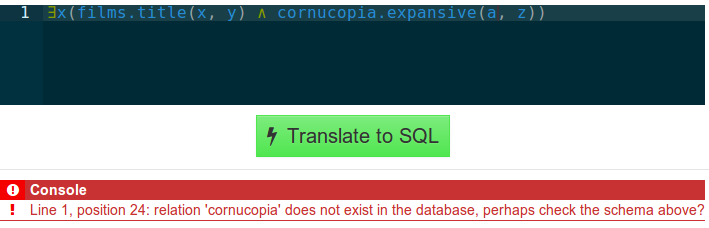
\includegraphics[width=1.0\textwidth]{images/error.png}
        \caption{A user being informed of a semantic error: the relation
          'cornucopia' does not exist in the schema.}
      \end{figure}

    \subsubsection{Error Handling}
      There were many stages of the translation process which could have
      encountered errors that needed to be sent back to the user. To deal with
      this, an exception-based error reporting system was created.

      The basic idea behind this was to put each stage of the translation in a
      \texttt{try: catch:} block. Then, if a stage encountered a problem it
      would raise exceptions containing the error information, which would cause
      the relevant \texttt{catch:} block to be called. This block would then add
      the exception as a Python dictionary to the AJAX response, and when sent
      back to the UI as JSON it would be able to construct a useful error
      message based on the exception data.

      Therefore, a Python exception class was created for each type of error
      that could be produced, containing all the relevant information about the
      error. Additionally, a special exception group class had to be created to
      allow the raising of multiple exceptions by any stage of the translation
      process (Python can only raise a single exception at a time).

      In the UI, if the `status' string of the AJAX response is not ``ok'', this
      indicates an error response. In this case the value is switched upon based
      on various error status codes, for example `parse\_error', and the `error'
      member of the response is then interpreted accordingly. This involves
      displaying an error line in the `console' section of the HTML page for
      each exception returned by the back end.

  \subsection{Testing}
  To ensure the reliability of our software we needed a testing framework that
  we could run easily. We chose to write standard Python unittest tests and on
  top of these used the nose testing framework to call and profile the runs.
  Using nose gave us a clear indication of how many of our tests have passed
  and gave us an idea of how our system was performing.

  We also used paste, which is a set of libraries that allow you to autoate
  tests which interact with a web page. This gave us the ability to test
  sending requests from our interface, simulating user interactions in a
  repeatable and fast manner.


\section{Evaluation}

    We used several metrics to evaluate usability and performance of our project
    \subsection{User Interface}
    The usability of our site was of paramount importance, as one of our main
    use cases was for the project to be used as a teaching tool. In order to try
    and quantify each users interaction with our project we collected metrics
    such as, length of inputted queries over time (are they getting more
    complex?) and validity of the queries.

    \begin{minted}{python}
      # Profiling code to record query length versus time taken
      # for the user to enter it
      statistics = {'query_length': len(logic_to_translate),
                    'error': error,
                    'time to enter query': form.time.get_value()}

    \end{minted}
    
    \subsection{Application Performance Analysis}

    Because the response time per query would be a large factor in a user's
    experience of the site, we were very interested in recording the performance
    of each component of our site. We were able to quantify the final
    performance of our product at the end of the project, by calculating the
    average time to process each query.

    We used the python testing framework Nose with the '--with-profile' flag to
    figure out how long functions and sections of code were taking. 
    After profiling our code we found that queries to our database took a large
    percentage of time to run compared to the rest of the code (1.822s/2.307s =
    79\%) we worked to reduce its execution time, as this would yield the largest
    performance benefit for time spent working. 
    We modified our query() function so that it only read the connection 
    parameters for the database once, whereas it had previously been reloading 
    the  parameters from disk each time query() was called.  

    Towards the  end of the project we managed to cut the end-to-end response time 
    down to  around 1.5 seconds per query (ignoring network latency) which was 
    fast enough that the system felt qualitatively responsive. In order to obtain 
    this qualitative information, we used the online service SurveyMonkey to record 
    what users though with 71.4\% of users answering that the were "happy with speed
    of query processing", and 28.6\% not happy. 

    \subsection{Site Usability Improvements}
    Another insight we gained from our survey was that users wanted a tutorial
    or information page on the site to help them learn how to use the
    application. This was clear to see as over 70\% of users wanted such a
    system. In response we produced an information dialogue box which explained
    the key features and elements of the application.
    \todo{insert fig here}
    Survey results and information page implementation   
    \subsection{Testing Procedures}
    We used the testing framework Nose in order to rapidly develop test cases to
    ensure the correctness of our project. We employed TDD (write a failing
    test, write some code to make the test pass, refactor, repeat), and our group 
    members spent a considerable amount of time constructing test cases. Below is an 
    example test.
  
    \begin{minted}{python}
      @with_setup(setup_func, teardown_func)
      def test_select_one_from_one(self):
        logic = "?x(films.title(x, y))".decode('utf-8')-
        sql = "SELECT title FROM films"
        assert self.translates_to(logic, sql), "Error, expected answers not equal"
    \end{minted}

    In order to add new test cases our group all met together and hand translated 
    example logic queries and their SQL equivalents. By constantly adding new tests 
    based on queries that were either produced within our group, or suggested by our 
    supervisor and others, we quickly expanded our test cases to cover many of the 
    possible queries that a user could enter. At the time of writing we have 92 test 
    cases that pass each testing different constraints on our project.


 

\section{Project Management}
  \subsection{Planning}
    As we have learnt from previous projects, inside and outside the
    department, it is critical to thoroughly plan a software engineering
    exercise of this scale before beginning to implement features and write
    code. As discussed in our introduction section, we decomposed our problem
    of translating first order predicate logic to SQL into several key
    subgoals. This enabled us to outline a core feature set which we wished to
    implement and gave us a much clearer idea of how to begin tackling the
    problem.

    Moreover, we initially split the project up in to five major 'revisions'.
    Each revision added a certain amount of functionality to our project, and
    allowed us to continually build upon features already implemented. This
    incremental method of development is one of the key ideas of the Agile
    development methodology to which we adhered to throughout the project.
    \cite{agilemanifesto} Additionally, with each revision having a
    deadline, it gave the team a clear plan of what was to be implemented at
    what time.

    \begin{table}[H]
      \centering
      \begin{tabular}{| l | p{0.6\textwidth} | l |}
        \hline
        \textbf{Revision} & \textbf{Necessary Steps for Completion}
          & \textbf{Completion Estimate} \\
        % \multicolumn{1}{p{0.6\textwidth} |}{\textbf{}}
        \hline
        1 &
          \begin{compactitem}
            \item Set up basic web server;
            \item Set up and create a database;
            \item Create simple UI \& communicate with server;
            \item Create 5 sample Logic to SQL translations;
            \item Set up development environment.
          \end{compactitem}
          & 17/10/13 \\
        \hline
        2 &
          \begin{compactitem}
            \item UI sends predicate logic to web server;
            \item Web server parses the logic into an AST;
            \item Backend translates the AST to SQL for basic \texttt{SELECT
              FROM} queries (i.e. projection only);
            \item Create 5 more sample Logic to SQL translations.
          \end{compactitem}
          & 25/10/13 \\
        \hline
        3 &
          \begin{compactitem}
            \item Expand backend parser grammar to include more advanced use of
              SQL queries (selection \& projection);
            \item Dynamic table selection in logic - "smart" logic predicates,
              e.g. \texttt{updated(x)} vs. \texttt{customer.updated(x)};
            \item Hook into database.
          \end{compactitem}
          & 1/11/13 \\
        \hline
        4 &
          \begin{compactitem}
            \item User-defined functions;
            \item Configurable UI - database settings, and possibly changing the
              UI depending on the user's ability;
            \item Extend backend to use SQL joins.
          \end{compactitem}
          & 8/11/13 \\
        \hline
        5 &
          \begin{compactitem}
            \item Contingency time built in for bug fixes, or additional
              features/extensions depending on the project status (e.g. Semantic
              checks of logical statements before translating to SQL).
          \end{compactitem}
          & 15/11/13 \\
        \hline
      \end{tabular}
      \caption{Feature sets for each revision, as defined at the start of the
        project}
    \end{table}

    However, as can often happen in software engineering projects, the plan
    changed somewhat as the project progressed. It turned out that turning
    logical statements to intermediate representation would take longer than
    previously thought, and was not so simple to apply Agile iterations to. Due
    to the complexity of the translator, the group wanted to ensure that we
    had a solid structure in place that would support all of the logic features
    necessary. It would have been possible to write an IR generator that only
    supported basic features very quickly, but this would have reduced
    extensibility of the product. Therefore, we believe deviating from the plan
    was the right choice in this instance. Beyond this issue, the group on the
    whole stuck to the plan, and features were implemented on time - with ample
    time during the Christmas break for extensions.

  \subsection{Group Organisation}
    At the beginning of the project, as discussed previously, we outlined the
    goals and required features of our project, and split them up in to three
    rough areas - front end (handling user interactions),
    middle end (communicating between client and server), and
    then the back end (translation and database access).
    We initially split our group of six in to three teams,
    corresponding to each of the subsections of our project. Members were
    allocated to each team depending on their strengths - initially Ted and Tom
    were to complete front end work, Sam and Mitchell to do middle end, and
    Sean and Max on back end. These were just initial roles, and we found that
    throughout the project, roles could be temporarily switched around to put
    extra work in to tasks that took longer than expected.

    One of the key ways we kept our group organised was through weekly
    meetings.  During each weekly meeting, we discussed what tasks were to be
    completed that week, and spoke in detail about any concerns members had
    about the tasks that had been completed previously. We would also analyse
    the previous weeks performance, and make changes to our plan accordingly.
    This falls in line with a key principle of Agile development, where a team
    must be adapatable to change \cite{agilemanifesto}. 
    An example of such a change is when we realised implementing the parser 
    would take longer than originally thought. This lead us to modify our 
    feature set, reallocate group roles temporarily, and modify deadlines 
    and revision subgoals.

  \subsection{Tracking}
    Once an overarching plan was agreed on, we split each major goal of each
    revision in to smaller tasks. For each of these tasks, we then allocated a
    numerical estimate of the time it would take to complete, on a scale of 1
    to 5, where 1 signified a short task and 5 signified a very time consuming
    task. The estimate of time a task would take was initially based on
    previous experience on other software engineering projects the group
    participated in, but as the project progressed, we applied knowledge of how
    prior tasks went to more accurately assign estimates.

    A typical practice in Agile development is for developers to write down
    their tasks on cards, and then place them on a physical board (known as an
    "information radiator") located in sight of all developers on the project.
    Upon this board are "swim lanes"; columns which cards belong to, and denote
    their progress (e.g. "to do", "doing" and "done") \cite{agileswimlane}. 
    Each task has a time
    estimate (as discussed above), and is assigned to one or more people to
    complete.  This allows every developer to know exactly what is happening at
    what time, what has to be done, and what has been completed. For our group,
    working in DoC labs and at home, this would obviously not be practical.
    Therefore, we used web-based project management software called
    Trello\cite{trello}. This software behaves in the same way as a physical board, but is
    accessed via a web based interface which can be edited by all members of
    the project.  Additionally, each card has a hashtag which denotes which
    revision a task belongs to, or if a stricter deadline is required, a date
    for completion can be manually added.  Virtual cards are moved between each
    swim lane as the task progresses. The group found this tool indispensible
    for communication and keeping on track with the project.

    \begin{figure}[H]
      \centering
      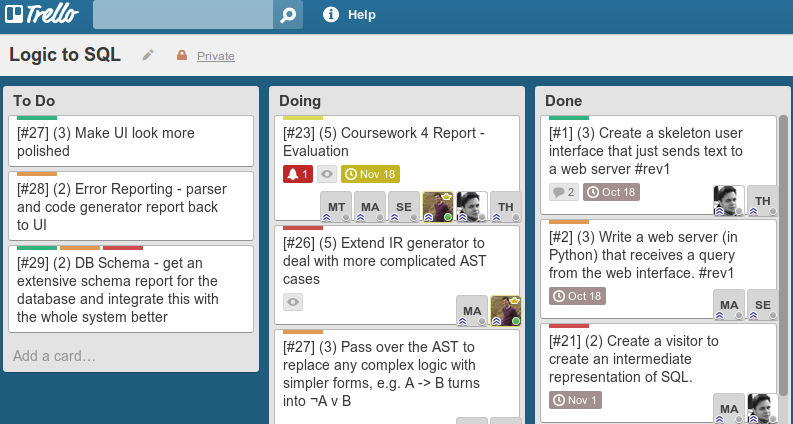
\includegraphics[width=0.9\textwidth]{images/trello.png}
      \caption{A screenshot of our Trello board toward the end of our project.}
    \end{figure}

  \subsection{Version Control}
    The group made use of the popular Git\cite{git} version control software.
    The choice of Git over other version control packages (e.g. Mercurial,
    Subversion, Perforce) was obvious for us; it's freely available, gets the
    job done, and all team members have strong experience with the software.
    Moreover, for hosting our repository, we used the department's GitLab
    server. This was to keep the source code within the department, low
    latency to the server from within labs, and to make use of CSG backups. The
    benefits of GitLab over a service like GitHub, however, were mostly
    marginal.

    Additionally, we made use of a script named
    github-trello\cite{githubtrello} to integrate our Trello board with our
    version control. This script allows Git commits to reference Trello cards
    and move them between swim lanes. For example, a commit containing the word
    "begin \#4" would move card number 4 from the "To Do" swim lane to the
    "Doing" swim lane. As this service only works with GitHub, one of our group
    members forked the project\cite{tedtrello} and extended its functionality 
    to work with GitLab, and also allow for multiple cards to be referenced per
    commit. The group found this functionality to be very useful, and it also
    reduced the likelihood that a member would forget to move a card from
    "Doing" to "Done", for instance.

  \subsection{Continuous Integration}

    As discussed earlier, we have an extensive test suite for which to test our
    code against throughout the development process, employing Test Driven
    Development (TDD). These tests can be run manually by typing
    \texttt{nosetests} on the terminal. However, we needed a way to automate
    this.

    Therefore, we decided to make use of the TeamCity \cite{teamcity}
    continuous integration server. The choice of TeamCity was made as the group
    deemed it to be the best package available; other CI servers such as
    Jenkins have a difficult-to-use interface, and another popular choice,
    Travis CI, only works with GitHub. TeamCity runs on our server,
    and monitors our Git repository for any changes on the 'testing' branch.
    When a change is detected, it runs our test suite on the code and, if the
    tests pass, the branch is merged in to the 'master' branch. If tests fail,
    a failure message is received and no merge occurs. Additionally, if the
    commit contains the tag '\#deploy', and all tests pass, then TeamCity 
    automatically pushes our code to our deployment server, where it is 
    accessible via the web. The use of TeamCity was useful in ensuring no
    broken code could be deployed, and to inform developers to inadvereant
    pushes of broken code.

    One issue that remains with this is that a group member may manually push
    code or try to merge code in to the 'master' branch. Only TeamCity should
    be able to do this, via the 'testing' branch. To prevent group members from
    violating this arrangement, we set up a Git hook script that aborts any
    attempted commits to 'master'. Additionally, a humorous message is
    displayed.

    \begin{figure}[H]
      \centering
      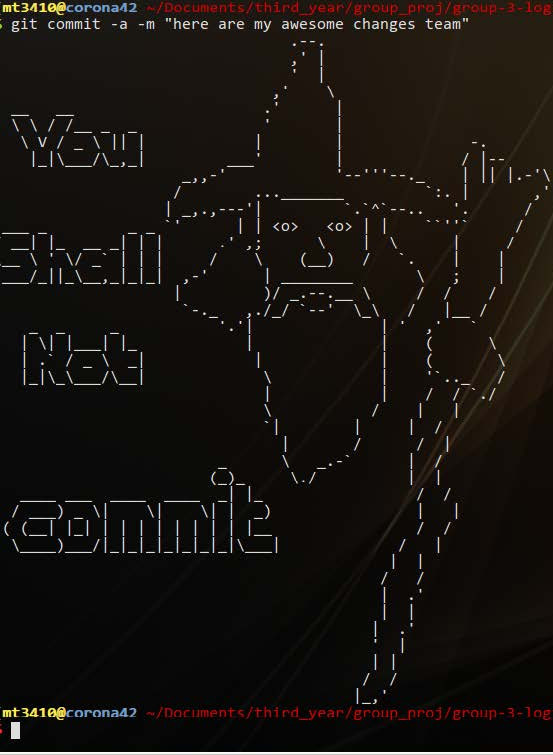
\includegraphics[width=0.3\textwidth]{images/gandalf.jpg}
      \caption{Gandalf informs the developer that they shall not commit.}
    \end{figure}

\section{Conclusion and Future Extensions}

  At the start of this project no member of the group had any significant
  experience programming in Python, despite this we found it very easy to pick
  up and learn on the fly. However this lead to some of the early code we
  wrote being refactored several times after learning significant features
  of the language which allowed us to simplify the code considerably, we found 
  the use of Python dictionaries to be invaluable, for example it allowed us to 
  rapidly build a well defined error handling system with minimal effort.
  
  
  One stumbling block we encountered was a lack of self documentation half way
  through the project. Upon reflection, at the beginning of the project we 
  started well, planning in advance and making sure team members were kept up 
  to date with the technical details of how the project worked. However as time 
  progressed this changed, there was a tendency for some members of the project 
  to work on an area without informing others of their intention, or specifying 
  abstractly how they were solving certain problems. For example at the beginning 
  of the project everybody had a good understanding of how we would parse the 
  grammar for predicate logic and how we could build up a syntax tree, but later 
  on during the codegen phase a few members (whilst doing sterling work) 'ran away'
  with the project resulting in a large chunk of code which only a few people
  understood; this greatly reduced how many people could contribute to that part
  of the project without spending a significant amount of time figuring out what
  that piece of code did, which in turn slowed down development of certain
  features while everyone took time to figure out how the project worked.
  Really what we have learnt from this is that documentation is key, indeed if the
  group were to do the project over again, we would have made sure that for each
  agile sprint a group member would be tasked solely with the role of 'Technical
  Writer' who's job it would be to produce a set of specifications for each part
  of the project worked on that week. 


  \subsection{Future Extensions}
    During the course of this project we did not get time to implement several
    features we had initially hoped to provide. 

    \subsubsection{Language Features}
    Initially we wanted to have a mechanism by which as user would be able to
    define the meaning of a predicate which they could then use in their query.
    This would help with creating quick shortcuts and cut down on the amount of 
    repeated logic a user would have to write. For example being able to define a 
    predicate \texttt{stars\_in(aname,ftitle)} which relates an actor with a name 
    'aname' staring in a film with title 'ftitle'
    \begin{align*}
      stars.in(aname, title) \models \exists  & f,c,a (  &                                    \\
                                              & films.title(f,title) \land &                  \\
                                              & casting.fid(c,f) \land &                      \\
                                              & casting.aid(c,a) \land &                      \\
                                              & actors.name(a,aname) &                        \\
    ) \hspace{2mm} & &
    \end{align*}

    Also currently we have no facility to express SQL operations like INSERT, 
    DROP, CREATE, UPDATE, and DELETE, we only operate on the 'read-only' part 
    of DML, there is a vast set of SQL which we are unable to provide a mapping 
    for in our system. Perhaps a set of special predicates could be defined in
    order to facilitate these operators.
    
    \subsubsection{Web Frontend Features}
    There are a few security issues with our project as it stands, currently our 
    project is vulnerable to several SQL injections. While working on the project
    we prioritised the translation task over the security of the system, if the 
    project were to be taken further these issues would need to be addressed. 
    Additionally, whilst the connection to our site is secured via HTTPS, 
    passwords to the database are still sent in 'plaintext' over HTTPS.
    

    There are a few niceities which would be useful to have but are not vital
    these are not limited too: increasing responsiveness of the system whilst 
    running long queries (providing the user feedback to let them know that the
    system hasn't crashed), saving a recent history of queries, developing a 
    tablet version of the site, being able to truncate the output of queries if 
    they are too long, caching results of recent queries to improve performance,
    and having a mechanism to download the results of a logic query.  

    
    \subsubsection{Backend Features} 
    We would have liked our project to be able to support several database
    implementations. Currently it only supports Postgres databases, we had
    planned support several other major implementations like MySQL and
    Microsoft SQL Server, however due to lack of time this feature was removed
    in favour of focusing on making sure that the logical translations produced
    were correct. 
   
    Currently there is no scope for type checking in the semantic analysis phase
    of the SQL generation,\todo{asdflas;d}

   
    

\section{Bibliography}
  \printbibliography

  --TODO Agree on referencing practice. The library recommends Harvard. --

  https://workspace.imperial.ac.uk/library/Public/Harvard\_referencing.pdf

\appendix
\section{Appendix}
  The appendix is optional, and does not count towards the 35 pages. It may
  contain thing like: User guide, installation instructions; more extensive
  design, testing, statistics etc.

  \subsection{Installation Guide}
    For installation of our logic to SQL translator, we strongly recommend
    starting with a vanilla installation of Ubuntu 12.04 LTS, for which a guide
    follows. If you wish to install on another operating system (it has been 
    confirmed to work on Ubuntu 13.10 and Mac OS X Mavericks),
    limited help is given.

    \begin{enumerate}
      \item Firstly, install dependencies via \texttt{apt-get}, or similar
        package manager for your system (e.g. \texttt{brew} for Mac):
        \begin{verbatim}
          sudo apt-get install python-dev python-pip python-pastescript
          python-nose postgresql libpq-dev libxml2-dev libxslt-dev
          rabbitmq-server openssl
        \end{verbatim}

      \item Secondly, install the required Python packages via \texttt{pip}.
        This should work regardless of platform (replace \texttt{sudo} with the
        command to elevate to superuser privileges for your platform):
        \begin{verbatim}
          sudo pip install psycopg2 celery lxml
        \end{verbatim}

      \item Extract the Logic to SQL project tarball to your desired
        installation folder.

        Now, modify \texttt{INSTALL\_DIR/dbbackend/db.cfg} for your PostgreSQL
        database. The format of this file is intuitive.

      \item The project requires an SSL certificate. The certificate
        files need to be in \texttt{INSTALL\_DIR/certs} with files
        \texttt{server.key, server.csr} and \texttt{server.crt}.

        To generate your own certificates, see:\\
        \url{http://chschneider.eu/linux/server/openssl.shtml} or the
        documentation at \url{http://www.openssl.org}

      \item \textbf{Optional}: If you decide to use
        the default database settings (the \texttt{filmdb} database), then you
        can test your installation by running our test suite. This runs
        our test suite to confirm your installation is configured correctly.
        Run the following in \texttt{INSTALL\_DIR}.

        First, type \texttt{python dbbackend/generate\_schema.py} to generate
        the schema for the test cases to use. Now. run \texttt{nosetests}. If
        all tests pass, your installation is configures correctly. Note that
        our test suite is only compatible with the \texttt{filmdb} database.

      \item The server can now be started by running the following:

        \begin{verbatim}
          celery --app=task worker &>> celery.log &
          ./run PORT_NUM &>> webpy.log &
        \end{verbatim}

        The software will now be accessible via
        \texttt{https://localhost:PORT\_NUM}. Logs will be available in
        \texttt{celery.log} and \texttt{webpy.log}. Note that if you wish to
        run the server on port 80, you must execute the \texttt{run} script
        with superuser privileges (i.e. with \texttt{sudo}).

        As the project is designed to run as a daemon, these commands can be
        added to a boot-up script. The processes may be terminated in the
        normal way.
    \end{enumerate}

  \subsubsection{Other Operating Systems and Dependencies}

  To install our project on other operating systems, the following dependencies
  must be met (including version tested with).

  \begin{itemize}
    \item Python, including dev tools (2.7.x) - \url{http://python.org}
    \item Pip (1.0) - \url{http://www.pip-installer.org/en/latest/}
    \item Nose (1.1.2) - \url{https://github.com/nose-devs/nose/}
    \item Paste (1.7.5.1) - \url{http://pythonpaste.org/}
    \item PostgreSQL (9.1) - \url{http://www.postgresql.org/}
    \item libpq-dev - \url{http://www.postgresql.org/}
    \item libxml2-dev - \url{http://www.xmlsoft.org/}
    \item libxslt-dev - \url{http://xmlsoft.org/XSLT/}
    \item RabbitMQ - \url{http://www.rabbitmq.com/}
    \item OpenSSL - \url{http://www.openssl.org/}
  \end{itemize}

  The installation then broadly follows step 2 and onwards from the above
  guide. 

  \textbf{Note:} We have determined an incompatability between our project and
  the Gentoo operating system. We make use of the RabbitMQ message server,
  which has a dependency on the Erlang language libraries. These libraries
  are notoriously difficult to install on Gentoo, as confirmed by a visit to
  the Erlang IRC channel.

  \subsection{Schemas}

    \subsubsection{Films Database - filmdb}
    \label{sec:appfilmdb}

      \begin{figure}[H]
        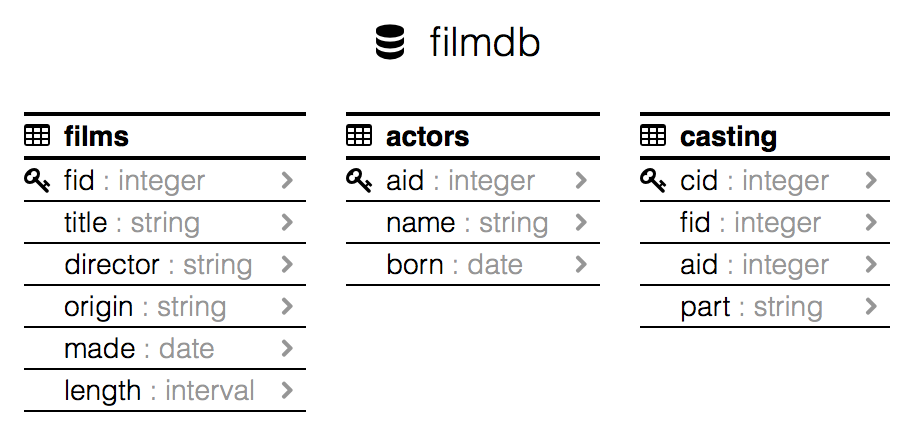
\includegraphics[width=\textwidth]{images/site_schema.png}
        \caption{Basic 'filmdb' schema, containing information about films,
        their actors, directors etc.}
      \end{figure}

      The films database is based upon the example database used in teaching
      the first year databases course.

    \subsubsection{Shakespeare Database - shakespeare}

      \begin{figure}[H]
        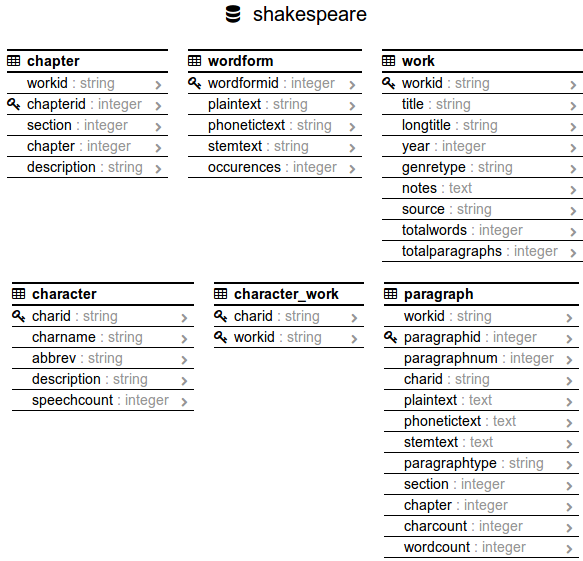
\includegraphics[width=\textwidth]{images/site_schema_shakespeare.png}
        \caption{More advanced 'shakespeare' schema, containing information
        about his literary works.}
      \end{figure}

      The Shakespeare database is taken from \\
      \url{https://github.com/catherinedevlin/opensourceshakespeare}, which
      itself is based on the Open Shakespeare Project, \\
      \url{http://www.opensourceshakespeare.org/}.

  \subsection{Example Queries}

  The following queries make use of the \texttt{filmdb} and
  \texttt{shakespeare} schemas, outlined above.

    \subsubsection*{"Get me all films, their titles, directors, and when they
      were made"}

      Logic:
      \begin{gather}
        \exists x(films.title(x, y) \land films.director(x, z) \land films.made(x, a))
      \end{gather}

      SQL Generated:
      \begin{minted}{sql}
        SELECT films.title, films.director, films1.made
        FROM films JOIN films AS films1 ON (films.fid = films1.fid) AND
        (films.fid = films1.fid)
      \end{minted}

      This demonstrates a redundancy in our code generator whereby a
      \texttt{JOIN} is performed unnecessarily. However, the query is still
      correct and produces the correct results.

    \subsubsection*{"Get me all actors and the roles they've played."}

      Logic:
      \begin{gather}
        \exists x,a(casting.part(x, y) \land casting.aid(x, a) \land actors.name(a, b))
      \end{gather}

      SQL Generated:
      \begin{minted}{sql}
        SELECT casting.part, actors.name
        FROM casting JOIN actors ON casting.aid = actors.aid
        WHERE (actors.aid = casting.aid) AND (actors.aid = casting.aid)
      \end{minted}

    \subsubsection*{"Get me directors where all their films are greater than 100
      minutes long."}

      Logic:
      \begin{multline}
        \exists x(films.director(x, dir) \land \forall y(films.director(y, dir)
        \\
        \to (films.length(y, len) \land len > '100')))
      \end{multline}

      SQL Generated:
      \begin{minted}{sql}
        SELECT films1.director
        FROM films AS films1
        WHERE NOT (EXISTS (SELECT films2.fid, films2.director, films2.length
        FROM films AS films2
        EXCEPT
        SELECT films2.fid, films2.director, films2.length
        FROM films AS films2
        WHERE ((films2.length > '100') AND (films2.director = films1.director))
        AND (films2.director = films1.director) ) )
      \end{minted}

      \subsubsection*{"Get me character names and descriptions for all
        characters in either 'Othello' or 'Macbeth', where the characters
      speaks over 50 lines."}

      Logic:
      \begin{multline}
        \exists cid,wid(character.charname(cid, name) \land character.description(cid,
        desc) \\
        \land character.speechcount(cid, sc) \land sc > 50 
        \land work.title(wid, play) 
        \\ \land character\_work(cid, wid) \land (play = 'Othello' 
        \lor play = 'Macbeth'))
      \end{multline}

      SQL Generated:
      \begin{minted}{sql}
        SELECT character.charname, character.description,
        character1.speechcount, work.title
        FROM character JOIN character AS character1 ON (character.charid =
        character1.charid) AND (character.charid = character1.charid) CROSS
        JOIN work JOIN character_work ON (((character.charid =
        character_work.charid) AND (character.charid = character_work.charid))
        AND (character1.charid = character_work.charid)) AND (work.workid =
        character_work.workid)
        WHERE ((character1.speechcount > 50) AND (NOT ((NOT (work.title =
        'Othello' )) AND (NOT (work.title = 'Macbeth' )) ))) AND
        ((character_work.charid = character.charid) AND (character_work.workid
        = work.workid))
      \end{minted}

      This query is easier to express in our logical syntax than it is in SQL.
      However, this query does show how SQL optimisations could be applied
      before returning the query to the user, although in practice, the SQL
      server would do such optimisations before execution.

  \subsection{UML Diagram}

  - Look online to see if this can be generated by any tools.

  - Or make a reduced one, just showing main components of the project e.g.
  parser, sql generator, semantic analyser, etc

  \subsection{Design Diagrams}
    \subsubsection{UML Diagram}
    \begin{figure}[H]
        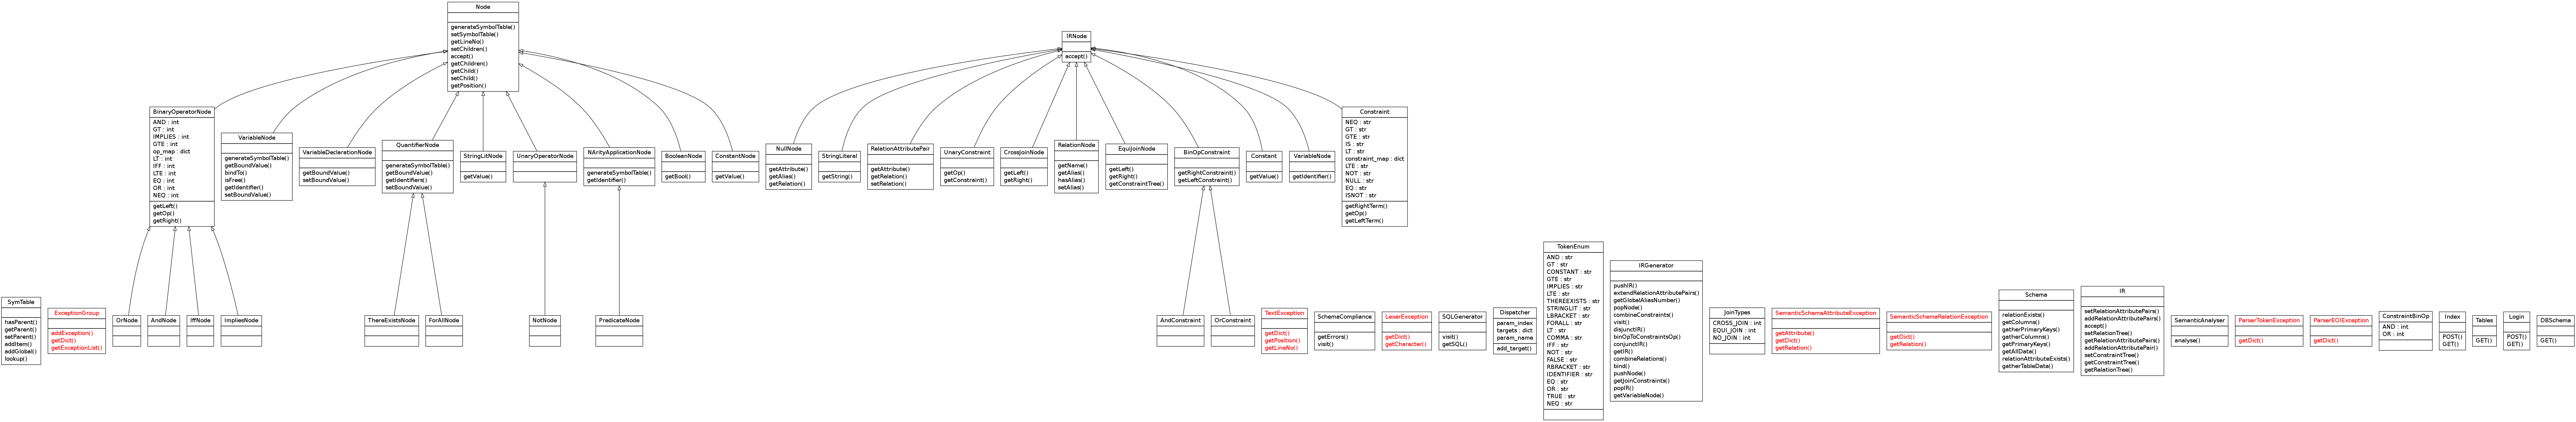
\includegraphics[width=1.0\textwidth]{images/umlisloveley.png}
        \caption{UML Diagram}
      \end{figure}

  - things like sean's bullshit rough drawings from Chatley reports

  \subsection{Statistics}

  - This is just the performance metric, profiling etc diagrams from 
  Chatley coursework 4.

%\section{Anandha waffle from his site - delete once finished report}
%  Final Report ? due: 13th Jan 2014, at 16:00 (both Electronic and Hardcopy)
%
%  Contents for Final Report: The project report should not be longer than 35
%  pages (recommended length is around 30 pages), and might be organised
%  according to the following structure: see above sections
%
%  Make sure that the final report presents a coherent story. Ask advice from
%  your supervisor. You might also draw inspiration from the instructions about
%  writing up your individual project.
%
%  Bear in mind, that most of the project assessors will not have followed the
%  project throughout and will only have a short time to listen to a
%  presentation or see a demonstration. For this reason they will rely heavily
%  on the report to judge the project.
%
%  The report should be submitted to SGO in form of a hard copy, as well as
%  electronically through CATE. i.e. report.pdf. 
%
%  ------------------------
%
%  Assessment
%  Will be updated soon.
%
%  Group project
%  The group project assessment is undertaken by each group's supervisor, and
%  moderated by a larger group of assessors, who will attend your presentation,
%  and/or read your final report. The assessment is based on:
%
%      Executive Summary, 5
%      Presentation, 10
%      Group Collaboration and Management, 20
%      Report, 30
%      Technical Achievement, 35
%
%  The group project (along with the Software Engineering course) is worth 440
%  Marks for both the MEng and BEng students.
%  Overall assessment
%  The overall assessment is the sum of the group project component and the
%  Software Engineering Course in an 80:20 split.
%
\end{document}
